\documentclass[11pt,letterpaper]{article}

\makeatletter
\renewcommand\paragraph{\@startsection{paragraph}{4}{\z@}%
                                      {1ex \@plus1ex \@minus.2ex}%
                                      {-1em}%
                                      {\normalfont\normalsize\bfseries}}
\makeatother

%%%%%%%%%%%%%%%%%%%%%
%  P A C K A G E S  %
%%%%%%%%%%%%%%%%%%%%%

% Authors
\usepackage{authblk}

% Page margins
\usepackage[margin=1in]{geometry}

% Nicer math font
\usepackage{mathpazo}

% More fancy lists
\usepackage{enumerate}

% Microtype
\usepackage{microtype}

% TikZ
\usepackage{tikz}
%\usetikzlibrary{calc,shapes.geometric}
\usetikzlibrary{backgrounds,fit,decorations.pathreplacing,calc}

% Highlights
\usepackage{soul}

% Young Tableaux
\usepackage{ytableau}

% Figure
\usepackage{float}

% Hypertext package
\usepackage[colorlinks = true]{hyperref}
% Title and authors
%\hypersetup{
%  pdftitle = {},
%  pdfauthor = {}
%}
% Color definitions
\definecolor{darkred}  {rgb}{0.5,0,0}
\definecolor{darkblue} {rgb}{0,0,0.5}
\definecolor{darkgreen}{rgb}{0,0.5,0}
% Color links
\hypersetup{
  urlcolor   = blue,         % color of external links
  linkcolor  = darkblue,     % color of internal links
  citecolor  = darkgreen,    % color of links to bibliography
  filecolor  = darkred       % color of file links
}

% AMS
\usepackage{amsmath,amssymb,amsfonts,amsthm,amstext}

%% Restating theorems
%\usepackage{thm-restate}

% Powerful macros
\usepackage{etoolbox}

% Fixes for amsmath
\usepackage{mathtools}
\mathtoolsset{centercolon}
\makeatletter
\protected\def\tikz@nonactivecolon{\ifmmode\mathrel{\mathop\ordinarycolon}\else:\fi}
\makeatother

% Daw boxes
\usepackage{tcolorbox}

% Code
\usepackage{algorithm}
%\usepackage{algorithmic}
\usepackage{algpseudocode}

% Clever references
\usepackage{cleveref}%[nameinlink]
\crefname{lemma}{Lemma}{Lemmas}
\crefname{proposition}{Proposition}{Propositions}
\crefname{definition}{Definition}{Definitions}
\crefname{theorem}{Theorem}{Theorems}
\crefname{conjecture}{Conjecture}{Conjectures}
\crefname{corollary}{Corollary}{Corollaries}
\crefname{claim}{Claim}{Claims}
\crefname{section}{Section}{Sections}
\crefname{appendix}{Appendix}{Appendices}
\crefname{figure}{Fig.}{Figs.}
\crefname{table}{Table}{Tables}
% \crefname{algorithm}{Algorithm}{Algorithms}

% IEEE tools
\usepackage[retainorgcmds]{IEEEtrantools}

% table of contents
\usepackage{tocloft}

% Table with multi-row
\usepackage{multirow}

% TikZ
\usepackage{tikz}	
\usetikzlibrary{backgrounds,fit,decorations.pathreplacing}

%%%%%%%%%%%%%%%%%%%%%%%%%
%  N E W C O M M A N D  %
%%%%%%%%%%%%%%%%%%%%%%%%%

% Standard quantum notation

\newcommand{\ket}[1]{|#1\rangle}
\newcommand{\bra}[1]{\langle#1|}
\newcommand{\braket}[2]{\langle#1|#2\rangle}
\newcommand{\ketbra}[2]{|#1\rangle\langle#2|}
\newcommand{\proj}[1]{|#1\rangle\langle#1|}

\newcommand{\x}{\otimes}
\newcommand{\xp}[1]{^{\otimes #1}}
\newcommand{\op}{\oplus}

\newcommand{\ct}{^{\dagger}}
\newcommand{\tp}{^\intercal}

% Linear algebra

%\newcommand{\1}{\mathbb{1}} % identity matrix
%\DeclareMathOperator{\Hom}{Hom}
\DeclareMathOperator{\End}{End}
%\DeclareMathOperator{\E}{\mathbb{E}}
\DeclareMathOperator{\Lin}{L} % all linear maps
\newcommand{\Mat}[1]{\mathrm{M}(#1)} % all matrices
%\newcommand{\Mat}[1]{\mathrm{M}_{#1}(\C)}

% Paired delimiters

\DeclarePairedDelimiter{\set}{\lbrace}{\rbrace}
\DeclarePairedDelimiter{\abs}{\lvert}{\rvert}
\DeclarePairedDelimiter{\norm}{\lVert}{\rVert}
\DeclarePairedDelimiter{\of}{\lparen}{\rparen}
\DeclarePairedDelimiter{\sof}{\lbrack}{\rbrack}
\DeclarePairedDelimiter{\ip}{\langle}{\rangle}
\DeclarePairedDelimiter{\floor}{\lfloor}{\rfloor}

% Operators

\renewcommand{\Re}{\operatorname{Re}}
\renewcommand{\Im}{\operatorname{Im}}
\DeclareMathOperator{\vc}{vec}
\DeclareMathOperator{\spn}{span}
\DeclareMathOperator{\rank}{rank}
\DeclareMathOperator{\diag}{diag}
\DeclareMathOperator{\spec}{spec}
\DeclareMathOperator{\Tr}{Tr}
\DeclareMathOperator{\sgn}{sgn}
\DeclareMathOperator{\hook}{hook}
\DeclareMathOperator{\E}{\mathbb{E}}
\DeclareMathOperator{\supp}{supp}


% Sets

\newcommand{\C}{\mathbb{C}}
\newcommand{\R}{\mathbb{R}}
\newcommand{\N}{\mathbb{N}}
\newcommand{\Z}{\mathbb{Z}}
\newcommand{\calH}{\mathcal{H}}
\newcommand{\calX}{\mathcal{X}}
\newcommand{\calY}{\mathcal{Y}}
\newcommand{\calA}{\mathcal{A}}
\newcommand{\calB}{\mathcal{B}}

% Group
\newcommand{\Zd}{\Z_d^{\times}}


% Identity operator
\newcommand{\1}{\mathbb{1}}

% Pauli Group
\newcommand{\Pg}{\mathcal{P}}
\newcommand{\J}{\mathcal{J}}

% Special notation

\newcommand{\CHSH}{CHSH^{(d)}}
\newcommand{\MS}{MS}
\newcommand{\SVT}{SVT}
\newcommand{\EPR}[1]{\Sigma^{(#1)}}
\newcommand{\paulix}{\sigma_x}
\newcommand{\pauliz}{\sigma_z}
\newcommand{\G}{G}
\newcommand{\LS}{LS}
\newcommand{\tM}{\tilde{M}}
\newcommand{\tN}{\tilde{N}}
\newcommand{\tA}{\tilde{A}}
\newcommand{\tB}{\tilde{B}}
\newcommand{\tX}{\tilde{X}}
\newcommand{\tZ}{\tilde{Z}}
\newcommand{\tU}{\tilde{U}}
\newcommand{\tW}{\tilde{W}}
\newcommand{\tx}{\tilde{x}}
\newcommand{\tpsi}{\tilde{\psi}}
\newcommand{\tri}{\Delta}
\newcommand{\lB}{\overline{B}}
\newcommand{\dr}[1]{d^{(#1)}}
\newcommand{\nr}{n(r)}
\newcommand{\mr}{m(r)}
\newcommand{\ux}{\underline{x}}
\newcommand{\uc}{\underline{c}}
\newcommand{\ua}{\underline{a}}


% Probabilities
\newcommand{\pr}[2]{P(#1|#2)}
\newcommand{\pa}[2]{P_A(#1|#2)}
\newcommand{\pb}[2]{P_B(#1|#2)}
\newcommand{\tpr}[2]{\tilde{P}(#1|#2)}

% Bell Ineqaulities
\newcommand{\I}{\mathcal{I}}

% Square root of epsilon
\newcommand{\ep}{\epsilon}
\newcommand{\se}{\sqrt{\epsilon}}
\newcommand{\qe}{\epsilon^{1/4}}
\newcommand{\sd}{\sqrt{d}}
\newcommand{\sr}{\sqrt{r}}
\newcommand{\qd}{d^{1/4}}

% Approximately equatli
\newcommand{\appd}[1]{\simeq_{#1}}

% Comments
\def\carl#1{{\color{blue} #1 -Carl}}
\newcommand{\hf}[1]{\textcolor{red}{#1}}

%%%%%%%%%%%%%%%%%%%%%%%%%
%  N E W T H E O R E M  %
%%%%%%%%%%%%%%%%%%%%%%%%%

\newtheorem{theorem}{Theorem}
\newtheorem{lemma}[theorem]{Lemma}
\newtheorem{proposition}[theorem]{Proposition}
\newtheorem{definition}[theorem]{Definition}
\newtheorem{corollary}[theorem]{Corollary}
\newtheorem{conjecture}[theorem]{Conjecture}
\newtheorem{claim}[theorem]{Claim}
\newtheorem*{conjecture*}{Conjecture}
\newtheorem*{problem}{Problem}
\newtheorem*{example}{Example}

\theoremstyle{definition}
\newtheorem*{remark}{Remark}



%%%%%%%%%%%%%%%%
%   Document   %
%%%%%%%%%%%%%%%%

\begin{document}

\title{Robust self-testing of large entanglement with constant alphabet}

\author[1]{Honghao Fu}
\author[1,2]{Carl Miller}

\renewcommand\Affilfont{\itshape\small}



\affil[1]{Department of Computer Science, Institute for Advanced Computer Studies, and Joint Center for Quantum \break Information and Computer Science, University of Maryland, College Park, MD 20742, USA}
\affil[2]{National Institute of Standards and Technology, 100 Bureau Dr., Gaithersbug, MD 20899, USA}
\maketitle

%========================================
\section{Introduction}
\label{sec:intro}
%========================================
Self-testing is a unique phenomenon of quantum mechanics. It has many applications in quantum
delegated computation \cite{ruv2013,cgsv2017} and device independent quantum cryptography
\cite{qkd2011,qkd2014,miller2016,fu2018,eat2018}.

The case of self-testing $2$-dimensional EPR pair is fully understood. One can robustly self-test
one copy of it by the CHSH inequality \cite{bamps2015}. and self-test many copies of the $2$-dimensional EPR
pair in parallel \cite{mckague2016, coladan2017parallel}. 
Self-testing general $d$-dimensional EPR pairs is a harder task.
Recently, a remarkable result by Coladangelo \textit{et al}.\cite{cgs2017} 
has shown that the maximally entangled state with arbitrary local dimension 
can be self-tested with constant question alphabet but answer alphabet growing with
the local dimension. 
Then Coladangelo and Stark \cite{coladan2017} further showed that by playing many instances
of the generalized Magic Square game and Magic Pentagram game, one can robustly self-test
$N$ copies of the maximally entangled state with local dimension $d$ for any $d, N \geq 2$.
Both the Magic Square game and the Magic Pentagram game have constant question alphabet
but answer alphabet of size $d$.

At a high level, general $d$-dimensional maximally entangled states are self-tested by
modifying the correlation and enlarging the size of the correlation.
A natural question to ask is whether maximally entangled state with large local dimension
can be self-tested with fixed-sized correlation. 
An equivalent question to ask is whether it is possible to self-test maximally
entangled state of some local dimension more efficiently, with constant correlation size. 
In this report, we give an affirmative answer to this question by proving the following theorem.
\begin{theorem}[Informal]
\label{thm:inf}
	There exists an infinite-sized set $D$ of odd prime numbers such that, for any $d \in D$, 
	the maximally entangled state of local dimension $d-1$ can be self-tested 
	with constant-sized question and answer alphabets.
\end{theorem}

The set $D$ is easily characterizable as it contains all the odd prime numbers with smallest
primitive root $2$, $3$ or $5$. It has been shown that there are infinitely many prime numbers
with smallest primitive root in the set $\{2,3,5\}$ \cite{murty1988}, so the set $D$ has infinitely many elements.
To prove \cref{thm:inf}, we give explicit self-testing proof of 
the maximally entangled state with local dimension $d-1$ where the primitive root of $d$ is $2$,$3$, or $5$, 
by explicitly giving the correlation that achieves self-testing. 
%Then the self-testing property of this correlation is 
%given in the following theorem.
%\begin{theorem}[Informal]
%\label{thm:pr_2}
%	All maximally entangled state with local dimension $d-1$, where $d$ is prime and has
%	primitive root $r \in \{2, 3, 5\}$, can be self-tested by a constant-sized correlation.
%\end{theorem}
Our correlation is denoted by $C(\dr{r})$ for prime $d$.
We use the superscript $(r)$ to denote the primitive root of $d$.
Note that although the size of $C(\dr{r})$ does not depend on $d$, the optimal correlation does.


In order to accomplish our goal, we introduce new techniques for self-testing.
First of all, we use a different variant of the weighted CHSH inequality, \hf{which was first introduced in \cite{acin2012}}, to enforce the eigenvalue of
some unknown operator which is the product of two binary observables used in the weighted CHSH test.
The variant of the CHSH inequality that we use is not used in the self-testing literature before.
Secondly, we give a new way to decompose unitaries of arbitrary order into binary observables which maintains
certain commutation relations. Such decomposition is different from what Slofstra used in his work \cite{slofstra2017}.
\carl{Our work is heavily based on \cite{slofstra2017}, and we need to make that clearer.}
Intuitively, such decomposition can be seen as the inverse of the Jordan's lemma decomposition.
The third contribution is that we prove self-testing without using anti-commutation relations between Pauli operators, 
which is the core idea in \hf{most of} the previous self-testing results.
\carl{Are we sure about that ("all")?}
Instead, we find a new pair of operators that can generate the ring of matrices over complex numbers.


\textbf{Structure of the paper}.
We start with notations and background information in \cref{sec:prelim}.
Since the correlation we designed can win a special linear system game and satisfy
an extended weighted CHSH test, we introduce the linear system game
in \cref{sec:lsg} and the extended weighted CHSH test in \cref{sec:chsh}. 
Our main result is based on the combination of the two tests and presented in \cref{sec:main}. 

%========================================
\section{Preliminaries and notations}
\label{sec:prelim}
%========================================
%-----------------------------------
\subsection{Notations}
%-----------------------------------
The maximally entangled state of local dimension $d-1$ for some odd prime $d$ that we are interested in is denoted by
\begin{align}
\ket{\EPR{d-1}} = \frac{1}{\sqrt{d-1}} \sum_{j = 1}^{d-1} \ket{j}\ket{d-j}.
\end{align}
The superscript $(d-1)$ stresses the dimension of the local Hilbert space and we follow this convention through this paper.
We denote a Hilbert space by $\calH$. Note that we only work with finite Hilbert spaces in this work.
When there are multiple Hilbert spaces, we label them with subscripts, for example, $\calH_A$ and
$\calH_B$.
The $d$-th root of unity is denoted by $\omega_d:=e^{2\pi i/d}$. In the qubit case, 
the maximally entangled state is denoted by 
\begin{align}
	\ket{\EPR{2}} = \frac{1}{\sqrt{2}}(\ket{00} + \ket{11}),
\end{align}
and the Pauli operators are given by
\begin{align}
	\paulix = \ketbra{0}{1}+\ketbra{1}{0} && \pauliz = \ketbra{0}{0} - \ketbra{1}{1}.
\end{align}

For quantum states and operators on different Hilbert spaces, we use subscripts to label them.
For example, $O_A$ is an operator on Alice's side and $\ket{0}_{B}$ is a state on Bob's side. 
The only exception is for projectors used in a quantum strategy defined below, where the subscript 
is the input and the superscript is the output. For example, $M_x^a$ is Alice's projector for input $x$ and output $a$.
Operators defined by the projectors follow the same convention, for example, $M_x := M_x^0 - M_x^1$.

We use the following notation for the closeness between quantum states.
\begin{align}
	\ket{u} \appd{\epsilon} \ket{v} \iff \norm{\ket{u} - \ket{v}} \leq \epsilon. 
\end{align}
Similarly, for numbers $a,b \in \C$, the closeness is denoted by
$a \appd{\epsilon} b \iff \norm{a-b} \leq \epsilon$.

We use some basic number theory in our work. 
\begin{definition}
A primitive root of a prime number
$d$ is \hf{the smallest integer} $r$ such that $r \pmod{d}$ has multiplicative order $d-1$
in the multiplicative group of integers modulo $d$, $\Zd$.
\end{definition}
In other words,
$r$ is the generator of $\Zd$.



%We self-test $\ket{\EPR{d-1}}$ by verify that Alice and Bob has operators
%\begin{align}
%	X = \sum_{k=1}^{d-1} \omega_d^k\ketbra{k}{k} && U = \sum_{k=1}^{d-1} \ketbra{k/r}{k},
%\end{align}
%where $\omega_d = e^{i2\pi/d}$ is the primitive $d$-th root of unity,
%and $r$ is the primitive root of $d$.  \carl{That sentence is jumping ahead --- you should just stick to
%definitions and notation for now.}
%Through out this paper, any operation on the label of the eigenvector $\ket{k}$ is taken modulo $d$,
%unless otherwise specified, for example, the $k/r$ above.
%-----------------------------------------
\subsection{Nonlocal games}
%-----------------------------------------
In a nonlocal game, there are two players, Alice and Bob and each of them is requested
to give an answer for a randomly chosen question. We denote Alice's question set by $\calX$ and her answer set by $\calA$. Similarly,
Bob's question set is denoted by $\calY$ and his answer set is denoted by $\calB$. The nonlocal game also
comes with two functions: $\pi: \calX \times \calY \rightarrow [0,1]$, which is the probability distribution over the questions,
and $V: \calA \times \calB \times \calX \times \calY \rightarrow \R$, which is the scoring function. 
Note that in the literature, the typical scoring function of a nonlocal game maps the input-output
pair to $\{0,1\}$ which corresponds to losing and winning. 
Such games are nonlocal
because Alice and Bob cannot communicate after getting their questions but they may share some strategy beforehand. 

A quantum strategy of a nonlocal game presented in terms of projective measurements
consists of projective measurements $\{\{M_x^a\}_a\}_x$ on Alice's side, 
$\{\{N_y^b\}_b\}_y$ on Bob's side, and a shared state $\ket{\psi}$, where 
$(M_x^a)^2 = M_x^a = (M_x^a)^\dagger$ and $(N_y^b)^2 = N_y^b = (N_y^b)^\dagger$.
\carl{You need to put explicit labels on the quantum systems used by
Alice and Bob.  (Later on you seem to use ``$A$'' and ``$B$'' to refer to those systems, but those are also
the same letters you use for Alice's and Bob's measurements.  That's confusing.)}
\hf{Addressed in the notation part. --H.F}
Then Alice and Bob's quantum strategy produces the conditional probability distribution
\begin{align}
	\pr{ab}{xy} = \bra{\psi} A_x^a \x B_y^b \ket{\psi} \text{ for all } (a,b,x,y) \in \calA \times \calB \times \calX \times \calY,
\end{align}
\begin{definition}
	Given sets $\calX, \calY, \calA, \calB$, a correlation is a collection of conditional probability distributions
	$\{\pr{ab}{xy}: a \in \calA, b \in \calB\}_{x \in \calX, y \in \calY}$.
\end{definition}
A particular type of nonlocal games that we are interested in is called linear system games, which is defined below.
\begin{definition}[Linear system game]
 Let $H\ux = \uc$ be an $m \times n$ system of linear equations over $\Z_2 = \{0, 1\}$,
 where $H$ is an $m$-by-$n$ matrix with entries in $\Z_2$ and 
 $\uc$ is a length-$n$ vector with entries in $\Z_2$. 
 The associated linear system game involves two
 players Alice and Bob, where Alice is given an equation number $i \in \calX = \{1 \dots m\}$ and replies with $\ua \in \calA = \Z_2^{\times n}$,
 and Bob is given a variable number $j \in \calY = \{1 \dots n\}$ and replies with an assignment $b \in \calB = \Z_2$. The 
 scoring function is defined by
 \begin{align}
 	V(\ua, b, i, j) =
	\begin{cases}
		1, \quad \text{if } \sum_{k= 1}^n H(i,k) \ua(k) \equiv c(i) \pmod 2 \text{ and } \ua(j) = b \\
		0,  \quad \text{otherwise.}
	\end{cases}
\end{align}
\end{definition}
\carl{Make this clear in the definition itself.}
\hf{I made the definition of the scoring function part of the big definition now.}
In the later parts, we will work with quantum strategies for the linear system game presented in terms of binary observables.
\begin{definition}[Quantum strategy of a linear system game]
\label{def:q_strat}
A quantum strategy presented in terms of binary observables for the linear system game $(H\ux = \uc)$ consists of 
\begin{enumerate}
	\item a pair of finite Hilbert spaces $\calH_A$ and $\calH_B$;
	\item a collection of binary observables $B_j$, $1 \leq j \leq n$, on $\calH_B$
	such that $B_j^2 = \1$ for every $1 \leq j \leq n$;
	\item a collection of binary observables $A_{ij}$, $1\leq i \leq m$, $1\leq j\leq n$ 
	on $\calH_A$ such that 
	\begin{enumerate}
		\item $A_{ij}^2 = \1$ for every $i,j$,
		\item $\Pi_j A_{ij}^{H(i,j)} = (-\1)^{\uc(i)}$ for every $i$, and
		\item $A_{il}A_{ik} = A_{ik}A_{il}$ for every $i$ and $H(i,l) = H(i,k) =1$;
	\end{enumerate} 
	and
	\item a quantum state $\ket{\psi} \in \calH_A \x \calH_B$.
\end{enumerate}
\end{definition}
Note that any quantum strategy presented in terms of binary observables can be 
converted to a quantum strategy presented in terms of projective measurement by looking into
the spectral decompositions of the observables.

%It has been shown in Ref.~\cite{cleve2014} that the linear system game has a perfect strategy 
%satisfying conditions in \cref{def:q_strat} if and only if the linear system has a finite-dimensional
%operator solution in the following sense.  \carl{There's a missing reference here?}
%\begin{definition}[Operator solution of a linear system]
%\label{def:op_sol}
%	An operator solution to a linear system $Hx =c$ over $\Z_2$ is a sequence of \hf{finite-dimensional} Hermitian 
%	operators \hf{with finite entries}: $A_1, A_2, \dots A_n$ on a Hilbert space $\calH$ such that \carl{(What does the word ``bounded'' mean here?  It might
%	be best to just state the definition for finite dimensions only.)}
%	\begin{enumerate}
%		\item $A_i^2 = \1$, i.e. $A_i$ is a binary observable, for all $1 \leq i \leq n$;
%		\item If $x_l$ and $x_k$ appear in the same equation, then $A_l$ and $A_k$ commute;
%		\item for all $1 \leq i \leq m$,
%		\begin{align*}
%			\Pi_{k=1}^n A_k^{H(i,k)} = (-1)^{c(i)}\1.
%		\end{align*}
%	\end{enumerate}
%	A finite dimensional operator solution to a linear system $Hx = c$ over $\Z_2$ is an operator
%	solution in which the Hilbert space is finite-dimensional.
%\end{definition}
%Perfect quantum strategies can be extracted from operator solutions and vice versa.
A quantum strategy using binary observables for the linear system game associated with $H\ux = \uc$ can be constructed from
the finite-dimensional representation of a finitely presented group
over $\Z_2$, which is called the solution group.
\begin{definition}[Solution group of a linear system game]
	\label{def:presentation}
	Let $H\ux = \uc$ be an $m \times n$  linear system. The solution group of this system
	is the group
	\begin{align*}
		\Gamma(H,\uc) := \ip{
		x_1,\dots x_n, J: &J^2 = x_i^2 = e, Jx_i = x_iJ \text{ for all }1 \leq i \leq n, \\
				& \Pi_{j=1}^n x_j^{H(i,j)} = J^{\uc(i)} \text{ for all } 1 \leq i \leq m, \text{ and } \\
				& x_l x_k = x_k x_l \text{ if } H(i,k) = H(i,l) = 1 \text{ for some } i
				} .
	\end{align*}
\end{definition}
We remark that a linear system game can be extracted from a solution group and \textit{vice versa}.
Let $\Psi$ be a finite-dimensional representation of $\Gamma(H,\uc)$ such that $\Psi(J) = -\1$ on the vector space $\C^d$, then a prefect strategy for 
the linear system game ($H\ux = \uc$) has
\begin{enumerate}
	\item $A_{ij} = \Psi(x_j)$ for all $ 1 \leq i \leq m$ and $1 \leq j \leq n$,
	\item $B_j = \Psi(x_j)$ for all $1 \leq j \leq n$,
	\item the maximally entangled state $\ket{\psi} = \frac{1}{\sd} \sum_{k=1}^d \ket{k}\ket{k}$.
\end{enumerate}
We follow a similar approach to construct our ideal strategy. However, our strategy uses a different maximally entangled state,
so we justify our strategy more carefully.
For concepts related to group presentations, we refer to Sec.~$2$ of Ref.~\cite{slofstra2017}.
For concepts related to group representations, we refer to Sec.~$2.5$ of Ref.~\cite{coladan2017}.

%-------------------------------------------------------------------------------
\subsection{The weighted CHSH inequality \cite{acin2012}.}
%-------------------------------------------------------------------------------
The weighted CHSH inequality is extracted from the CHSH test, which is another nonlocal game. 
The input sets and output sets of Alice and Bob are
$\calX = \calY = \{1, 2\}$ and $\calA = \calB = \Z_2$.
The scoring function for the $\alpha$-weighted CHSH test is defined by
\begin{align}
	V(a,b,x,y)_{\alpha-CHSH} = 
	\begin{cases}
		\alpha (-1)^{a + b}, \quad \text{if } x = 1 \\
		(-1)^{a + b}, \quad \text{if } x = 2,\; y =1 \\
		(-1)^{1 + a + b}, \quad \text{if } x = y =2.
	\end{cases}
\end{align}
Let Alice and Bob's quantum strategy in terms of projectors be $( \{\{M_x^a\}_a\}_x, \{\{N_y^b\}_b\}_y, \ket{\psi})$. 
We define binary observables $M_x := M_x^0 - M_x^1$ and $N_y := N_y^0 - N_y^1$ from Alice and Bob's projectors.
The weighted CHSH inequality states that 
\begin{align}
	\label{eq:chsh_op}
	\ip{\I_\alpha} = \alpha\ip{M_1N_1}+\alpha\ip{M_1N_2} + \ip{M_2N_1} - \ip{M_2N_2}\leq 2\alpha,
\end{align}
where $\ip{M_xN_y} := \bra{\psi} M_xN _y \ket{\psi}$ is the expectation value of of the observables. 
The weighted CHSH inequality is true 
If Alice and Bob share product state $\ket{\phi} = \ket{\phi_A} \x \ket{\phi_B}$.
However, If they share an entangled state $\ket{\psi}$, the value of $\ip{\I_\alpha}$ can be as large as
\begin{align}
\label{eq:chsh_max}
 \ip{\I_\alpha}_{\max} = 2\sqrt{1+\alpha^2}.
\end{align}
\begin{definition}[Ideal strategy to achieve $\ip{\I_\alpha}_{\max}$]
	\label{def:ideal}
	Define $\mu = \arctan(1/\alpha)$.
	The ideal strategy for weighted CHSH with parameter $\alpha$, which achieves the value $\ip{\I_\alpha}_{\max}$, 
	consists of the joint state $\ket{\EPR{2}}$ and observables $\tM_1 = \pauliz$, $\tM_2 = \paulix$,
	$\tN_1 = \cos(\mu) \pauliz+ \sin(\mu) \paulix$ and $\tN_2 = \cos(\mu) \pauliz - \sin(\mu) \paulix$.
\end{definition}
An interesting observation of the weighted CHSH inequality is that if some strategy can achieve 
value $\ip{\I_\alpha}$ close to $\ip{\I_\alpha}_{\max}$, then the strategy is close to the ideal 
strategy up to some local isometry, 
which is a phenomenon referred as a robust self-test.
We give the formal statement of this self-testing property of $\ip{\I_\alpha}_{\max}$ in \cref{sec:chsh}.

\carl{Before the next definition, you should define what a ``correlation'' is.}
\hf{Done. I decided to remove the definition of self-testing here because I think it is hard
to give a general robust self-testing definition and it suffices to just give our robust self-testing result.}

\carl{Section 2 needs to be cleaned up in some places, but overall it is pretty good.}

%=======================================
\section{The linear constraint test}
\label{sec:lct}
%=======================================
In this section, we introduce a linear constraint test that is satisfied by our correlation.
The linear constraint test is designed to enforce relations that should be satisfied by 
Alice and Bob's observables and it is inspired by 
Slofstra's seminal work~\cite{slofstra2017}, in which he
embeds the group
\begin{align}
	K = \ip{ x,y,a,b:a^2=b^2=e, ab=ba, yay^{-1} = a, yby^{-1} = ab, xyx^{-1}=y^2}
\end{align}
into a linear system game such that the relations in the definition of $K$ can be derived from the
combination of the equations of the linear system game. Then he showed the difference between exact representations
and approximate representations of $K$, which implies that the set of quantum correlation is not closed.
\hf{We generalize the relation $xyx^{-1} = y^2$ and embed the 
following group}
\begin{align}
	G = \langle u, o : uou^{-1} = o^r \rangle, 
\end{align}
for some $r \in \N$ into a linear constraint test.

%------------------------------------------------------------------------
\subsection{The embedding of $G$}
%------------------------------------------------------------------------
The main result of this subsection is summarized in the following theorem.
\begin{theorem}
	The relation $uou^{-1} = o^r$ can be embedded in a linear constraint test which has
	$n(r) := 18r+86$ variables and $m(r) := 16r + 72$ equations, where each equation has $3$ variables.
\end{theorem}
We prove this by constructing the solution group $\Gamma$ of the linear constraint test. 
We also prove some properties of the generators of $\Gamma$ along the way.

We embed $G$ into $\Gamma$ in three steps and introduce two intermediate groups $G_0$ and $G_1$, which are defined below.
\begin{definition}
	The presentation of $G_0$ has order-$2$ generators:
	\begin{align}
		\{o_i\}_{i=1}^{r} \cup \{u_i\}_{i=1}^5
	\end{align}
	and relations:
	\begin{align}
	&u_3 = u_2o_1u_2 && u_4 = u_2o_2u_2 \\
	&u_5 = u_1u_3u_1 && o_2 = u_1u_4u_1\\
	&u_5 = o_1 o_r o_1,
	\end{align}
	and when $r$ is even
	\begin{align}
	&o_{1+2j} = o_1o_{2j}o_1 && o_{2+2j} = o_2o_{1+2j}o_2&& \text{ for } j = 1 \dots r/2 - 1;
	\end{align}
	when $r$ is odd
	\begin{align}
	&o_3 = o_2o_1o_2 &&
	 o_{2+2j} =o_1o_{1+2j}o_1 && o_{3+2j} = o_2o_{2j+2}o_2 &&\text{ for } j = 1 \dots (r-3)/2.
	\end{align}
\end{definition}
\begin{proposition}
	The group $G_1$ embeds the relation 
	\begin{align}
		(u_1u_2)^j o_1o_2 (u_2u_1)^j = (o_1o_2)^{r^j}, 
	\end{align}
	for any $ j \in \N$.
\end{proposition}
The proof follows the proof of Proposition~$4.8$ of Ref.~\cite{slofstra2017}
\begin{proof}
	We prove it by induction.
	Direct calculation gives us that
	\begin{align} 
		u_1u_2 o_1o_2 u_2u_1 = &u_1 (u_2 o_1u_2) (u_2o_2 u_2) u_1 \\
	=& (u_1 u_3 u_1) (u_1 u_4 u_1)\\
	=& u_5 o_2\\
	=& o_1o_ro_1 o_2.
	\end{align}
	Then substituting the definitions of $o_k$ for $k = r \dots 3$ gives us the case for $j=1$.
	
	Now assume the statement is true for $j = n$, then when $j = n+1$
	\begin{align}
		(u_1u_2)^{n+1} o_1o_2 (u_2u_1)^{n+1} =& u_1u_2 (o_1o_2)^{r^n} u_2u_1 \\ 
		 =& (u_1u_2 o_1o_2 u_2u_1)^{r^n} \\
		 =& (o_1o_2)^{r^{n+1}},
	\end{align}
	where from the first line to the second line, we insert $(u_2u_1)(u_1u_2)$ between every pair of $o_1o_2$ and $o_1o_2$.
	Hence, the statement is true.
\end{proof}
To better characterize all the conjugation relations above and simplify the form of $G_1$
and make the introduction of $G_2$ easier, we relabel $u_i$ and $o_i$'s
as $a_i$'s such that
\begin{align}
	a_j := 
	\begin{cases}
	 o_j \text{ for } j = 1,2 \\
	 u_{j-2} \text{ for } j = 3\dots 7 \\
	o_{j- 5} \text{ for } j = 8 \dots r+5.
	\end{cases}
\end{align}
Then we define the set $C(r)$ of tuples $(i,j,k)$ such that
\begin{align}
	(i,j,k) \in C(r) \iff a_ia_ja_i = a_k.
\end{align}
The size of $C(r)$ is $r+3$. 
%We can also employ some ordering of $C(r)$ such that $C(r,j)$ is a unique tuple for 
%$j = 1 \dots r+3$.
In this way, the group $G_0$ can be presented by
\begin{align}
	G_0  = \ip{ \{a_i\}_{i=1}^{r+5} : C(r) }.
\end{align}

Then we define the group $G_1$.
\begin{definition}
The presentation of $G_1$ has order-$2$ generators:
\begin{align*}
	\{a_i, b_i, c_i, d_i, v_i\}_{i=1}^{r+5}, f, g, \{h_{jk}\}_{(i,j,k) \in C(r)};
\end{align*}
and relations:
\begin{align*}
	&a_i = b_ic_i = fd_i = gv_i,&& fb_if =c_i &&\text{ for } i= 1 \dots r+5 \\
	&h_{jk}b_j c_k = e,&& d_ib_jd_i = c_k &&\text{ for all } (i,j,k) \in C(r).
\end{align*}
\end{definition}
Note that the group $G_1$ is slightly different from the group $K$ used in the proof of Lemma~$4.4$ of Ref.~\cite{slofstra2017}.
We introduce the generator $g$ so that later we can associate $f$ with $g$ in linear relations of the Magic Square game.
Such relations are important for the self-testing proof.
Two important properties of $G_1$ are given in propositions below.
The first property of $G_1$ was first proved in Lemma~$4.4$ of \cite{slofstra2017}.
\begin{proposition}
	The group $G_1$ embeds relation $x_ix_jx_i = x_k$ for all $(i,j,k) \in C(r)$.
\end{proposition}
\begin{proof}
	We first show that $d_i c_j d_i = b_k$, which is because
	\begin{align}
		d_i c_j d_i = d_i (f b_j f) d_i = f (d_i b_j d_i) f = f c_k f = b_k.
	\end{align}
	Then, we can prove that 
	\begin{align}
		a_i a_j a_i = f d_i b_j c_j f d_i = (f d_i b_j d_i f)(f d_i c_j d_i f) = (f c_k f)(f b_k f) = b_k c_k = a_k. 
	\end{align}
\end{proof}
\begin{proposition}
	In the group $G_1$, the generators $f$ and $g$ commute with $a_i$ for all $i = 1 \dots r+5$.
\end{proposition}
\begin{proof}
	We can check that
	\begin{align}
		fa_i f a_i = d_i d_i = e && g a_i g a_i = v_i v_i  = e,
	\end{align}
	for all $i = 1 \dots r+5$.
\end{proof}
Note that there are two types of conjugacy relations in $G_1$. One is of the form
$f b_i f = c_i$ for all $i = 1 \dots r+5$. The other one is of the form 
$d_ib_jd_i = c_k$ for all $(i,j,k) \in C(r)$. For each type of the conjugacy relations, 
we are going to embed it into a different set of linear relations in $\Gamma$.

\begin{definition}
\label{def:gamma}
The presentation of $\Gamma$ has order-$2$ generators:
\begin{align*}
	J, \{a_i, b_i, c_i, d_i, v_i,w_i,\{ k_{i,j} \}_{j=1}^5\}_{i=1}^{r+5}, \{f_i,g_i,m_i\}_{i=0}^2, \{h_{jk}\}_{(i,j,k) \in C(r)}, 
	\{\{ k_{c,j} \}_{j=1}^6\}_{c \in C(r)},
\end{align*}
and relations:
\begin{itemize}
\item for all $i = 1 \dots r+5$:
\begin{align}
	&a_i = b_ic_i = f_0d_i = g_0v_i \\
	&g_2 a_i w_i = e \\
	&f_0 f_1 f_2 = e && b_i f_2 k_{i,1} = e && k_{i,1} k_{i,2} k_{i,3} = e\\
	&f_0 k_{i,3} k_{i,4} = e && c_i k_{i,4} k_{i,5} =e && f_1 k_{i,2} k_{i,5} = e,
\end{align}
which embed $f_0 b_i f_0 = c_i$;
\item for all $ c = (i,j,k) \in C(r)$:
\begin{align}
	&h_{jk}b_j c_k = e\\
	&d_i k_{c,1} f_2 = e && b_j f_2 k_{c,2} = e && k_{c,2} k_{c,3} k_{c,4} = e\\
	&d_i k_{c,4} k_{c,5} = e && c_k k_{c,5} k_{c,6} =e && k_{c,1} k_{c,3} k_{c,6} = e,
\end{align}
which embed $d_i b_j d_i = c_k$;
\item relations of a Magic Square test:
\begin{align}
	&f_0 f_1 f_2 = e && g_0 g_1 g_2 = e &&m_0 m_1 m_2 = e \\
	&f_0 g_2 m_0 = e && f_2 g_0 m_1 = e && f_1 g_1 m_2 = J,
\end{align}
which embed $f_0 g_0 f_0 g_0 = J$ and $f_2 g_2 f_2 g_2 = J$;
\item $J$ commutes with all the other generators.
\end{itemize}
\end{definition}
The special properties of the generators of $\Gamma$ are summarized in the two propositions below.
\begin{proposition}
	The group $\Gamma$ embeds all the conjugacy relations of $G_1$.
	It also embeds the relations: $f_0 g_0 f_0 g_0 = J$ and $f_2 g_2 f_2 g_2 = J$.
\end{proposition}
The proof of the proposition above follows the proof of Proposition $4.2$ of Ref.~\cite{slofstra2017}.
\begin{proposition}
	In the group $\Gamma$, the generator $f_2$ commutes with $f_0$ and $a_i$ for all $i = 1 \dots r+5$;
	the generator $g_2$ commutes with $g_0$ and $a_i$ for all $i = 1 \dots r+5$.
\end{proposition}
\begin{proof}
	We show the commutativity property of $f_2$ as an example. The proof for $g_2$ is very similar.
	The commutativity between $f_0$ and $f_2$ is immediate from the relations.
	From the relation, we can also deduce that $f_2$ commutes with $b_i$ for all $i$.
	Since $a_i =b_ic_i = b_i f_0 b_i f_0$, we know $f_2$ commutes with $a_i$.
\end{proof}

%------------------------------------------------------------------------
\subsection{The representation of $\Gamma$}
%------------------------------------------------------------------------
In this section we give the presentation of $\Gamma$ which is built upon the representation 
$\Psi_0$ of $G_0$ and $\Psi_1$ of $G_1$. We need the representation of $\Gamma$ to construct the
ideal strategy that realizes our correlation.

Before giving the representation, we define two Hilbert spaces $W_{d-1}$ and $W_2$, which will form the carrier spaces
of the representations,
\begin{align}
	\label{eq:w_subspace}
	W_{d-1} := \spn(\{\ket{x_j}\}_{j=1}^{d-1}) && W_2 = \spn(\ket{x_1}, \ket{x_2}).
\end{align}
Note that another form of the basis of $W_{d-1}$ is $\{\ket{x_{r^j}}\}_{j=0}^{d-2}$, where the subscript $r^j$ is taken
modulo $d$ implicitly. We use the second form of the basis when it is convenient.
We denote the identity operator for these two spaces by $\1_{W_{d-1}}$ and $\1_{W_2}$.
On the Hilbert space $W_2$, we define
\begin{align}
	X_{W_2} = \ketbra{x_1}{x_2} + \ketbra{x_2}{x_1} &&
	Y_{W_2} = i\ketbra{x_1}{x_2} - i \ketbra{x_2}{x_1} &&
	Z_{W_2} = \ketbra{x_1}{x_1} - \ketbra{x_2}{x_2},
\end{align}
\begin{definition}
The representation, $\Psi_0$, of $G_0$ on $W_{d-1}$ is defined by
\begin{align}
	\Psi_0(a_1) =&\sum_{j=1}^{(d-1)/2} \omega_d^j \ketbra{x_j}{x_{d-j}} + \omega_d^{-j} \ketbra{x_{d-j}}{x_{j}} \\
	\Psi_0(a_2) = &\sum_{j=1}^{d-1} \ketbra{x_j}{x_{d-j}}\\
	\Psi_0(a_3) = &\ketbra{u_0}{u_0} +\omega_{d-1}^{(d-1)/2}\ketbra{u_{(d-1)/2}}{u_{(d-1)/2}}\\ + 
	&\sum_{k=1}^{(d-3)/2}\left( \omega_{d-1}^k\ketbra{u_k}{u_{d-1-k}} + \omega_{d-1}^{-k}\ketbra{x_{d-1-k}}{x_k}\right)\\ 
	\Psi_0(a_4) = &\ketbra{u_0}{u_0} +\ketbra{u_{(d-1)/2}}{u_{(d-1)/2}} \\+
	 &\sum_{k=1}^{(d-3)/2}\left(\ketbra{u_{d-1-k}}{u_k} + \ketbra{u_k}{u_{d-1-k}}\right),
\end{align}
where $\{ \ket{u_j} \}_{j=0}^{d-2}$ is a another basis of $W_{d-1}$ given by
\begin{align}
	\ket{u_k} = \frac{1}{\sqrt{d-1}} \sum_{j=0}^{d-2} \omega_{d-1}^{jk} \ket{x_{r^j}}.
\end{align}
The representation of the rest of the generators
can be constructed from $\Psi_0(a_1)$, $\Psi_0(a_2)$, $\Psi_0(a_3)$ and $\Psi_0(a_4)$ following the 
conjugation relations.
\end{definition}
We can check that
\begin{align}
	\Psi_0(a_1a_2) =  \sum_{j=0}^{d-2} \omega_d^{r^j} \ketbra{x_{r^j}}{x_{r^j}} &&
	\Psi_0(a_3a_4) =  \sum_{j=0}^{d-2} \ketbra{x_{r^{j-1}}}{x_{r^j}},
\end{align}
which satisfy the relation $\Psi_0(a_3a_4) \Psi_0(a_1a_2) \Psi_0(a_4a_3) = \Psi_0(a_1a_2)^r$ and
$[\Psi_0(a_3a_4), \Psi_0(a_2)] = \1_{W_{d-1}}$. 

Following the proof of Lemma~$4.4$ of Ref.~\cite{slofstra2017}, we construct a representation of $G_1$.
\begin{definition}
The representation $\Psi_1$ of $G_1$ on $W_2 \x W_{d-1}$ is defined by
\begin{itemize}
\item for $f_0$ and $g_0$
\begin{align}
	&\Psi_1(f_0) = X_{W_2} \x \1_{W_{d-1}} \\
	&\Psi_1(g_0) = Z_{W_2} \x \1_{W_{d-1}},
\end{align}
\item
for $i = 1 \dots r+5$,
\begin{align}
	&\Psi_1(a_i) = \1_{W_2} \x \Psi_0(a_i) \\
	&\Psi_1(b_i) = \ketbra{x_1}{x_1} \x \Psi_1(a_i) + \ketbra{x_2}{x_2} \x \1_{W_{d-1}} \\
	&\Psi_1(c_i) =\ketbra{x_1}{x_1} \x \1_{W_{d-1}} + \ketbra{x_2}{x_2} \x \Psi_1(a_i) \\
	&\Psi_1(d_i) =  X_{W_2} \x \Psi_0(a_i)\\
	&\Psi_1(v_i) = Z_{W_2} \x \Psi_0(a_i).
\end{align}
\item for $(i,j,k) \in C(r)$,
\begin{align}
	\Psi_1(h_{jk}) = \ketbra{x_1}{x_1} \x \Psi_1(a_j) + \ketbra{x_2}{x_2} \x \Psi_1(a_k).
\end{align}
\end{itemize}
\end{definition}

Finally, we follow the proof of Proposition $4.2$ of Ref.~\cite{slofstra2017} to construct the 
representation of $\Gamma$.
\begin{definition}
\label{def:rep_gamma}
The representation $\Psi$ of $\Gamma$ on $W_2 \x W_2 \x W_{d-1}$ is defined by:
\begin{itemize}
\item for any $x$ which is also a generator of $G_1$,
\begin{align}
	\Psi(x) = \1_{W_2} \x \Psi_1(x);
\end{align}
\item for the generators involved in the Magic square test
\begin{align}
	&\Psi(f_1) = X_{W_2} \x X_{W_2} \x \1_{W_{d-1}} \\
	&\Psi(g_1) = Z_{W_2} \x Z_{W_2} \x \1_{W_{d-1}} \\
	&\Psi(f_2) = X_{W_2} \x \1_{W_2} \x \1_{W_{d-1}} \\
	&\Psi(g_2) = Z_{W_2} \x \1_{W_2} \x \1_{W_{d-1}} \\
	& \Psi(m_0) = Z_{W_2} \x X_{W_2} \x \1_{W_{d-1}}\\
	& \Psi(m_1) = X_{W_2} \x Z_{W_2} \x \1_{W_{d-1}}\\
	& \Psi(m_2) = Y_{W_2} \x Y_{W_2} \x \1_{W_{d-1}}\\
	& \Psi(J) = - \1_{W_2} \x \1_{W_2} \x \1_{W_{d-1}};
\end{align}
\item for the generators $\{ w_i \}_{i=1}^{r+5}$:
\begin{align}
	\Psi(w_i) = Z_{W_2} \x \1_{W_{d-1}} \x \Psi_0(a_i);
\end{align}
\item for the generators to embed the relation $f b_i f = c_i$:
\begin{align}
	\Psi(k_{i,1}) &= X_{W_2} \x \Psi_1(b_i) = X_{W_2} \x ( \ketbra{x_1}{x_1} \x \Psi_0(a_i) + \ketbra{x_2}{x_2} \x \1_{W_{d-1}} )\\
	\Psi(k_{i,2}) &= \ketbra{x_1}{x_2} \x \Psi_1(b_if_0) + \ketbra{x_2}{x_1} \x \Psi_1(f_0b_i)\\
	&= \ketbra{x_1x_1}{x_2x_2} \x \Psi_0(a_i) + (\ketbra{x_1x_2}{x_2x_1}+\ketbra{x_2x_1}{x_1x_2})\x\1_{W_{d-1}}\\
	&+ \ketbra{x_2x_2}{x_1x_1} \x \Psi_0(a_i)\\ 
	\Psi(k_{i,3}) &= \ketbra{x_1}{x_1} \x \Psi_1(f_0b_if_0) + \ketbra{x_2}{x_2} \x \Psi_1(f_0) \\
	&= \ketbra{x_1x_1}{x_1x_1} \x \1_{W_{d-1}} + \ketbra{x_1x_2}{x_1x_2} \x \Psi_0(a_i) +  \ketbra{x_2}{x_2} \x X_{W_2} \x \1_{W_{d-1}}\\
	\Psi(k_{i,4}) &=  \ketbra{x_1}{x_1} \x \Psi_1(b_ic_i) + \ketbra{x_2}{x_2} \x \1_{W_2} \x \1_{W_{d-1}}\\
	&=(\ketbra{x_1x_1}{x_1x_1}+  \ketbra{x_1x_2}{x_1x_2}) \x \Psi_0(a_i) +  \ketbra{x_2}{x_2} \x \1_{W_2} \x \1_{W_{d-1}}\\
	\Psi(k_{i,5}) &= \ketbra{x_1}{x_1} \x \Psi_1(b_i) + \ketbra{x_2}{x_2} \x \Psi_1(c_i) \\
	&=\ketbra{x_1x_1}{x_1x_1} \x \Psi_0(a_i) + (\ketbra{x_1x_2}{x_1x_2} + \ketbra{x_2x_1}{x_2x_1}) \x \1_{W_{d-1}}\\
	&+ \ketbra{x_2x_2}{x_2x_2} \x \Psi_0(a_i);
\end{align}
\item for the generators to embed the relation $d_i b_j d_i = c_k$:
\begin{align*}
	\Psi(k_{c,1}) &= X_{W_2} \x \Psi_1(d_i) = X_{W_2} \x X_{W_2} \x \Psi_0(a_{i}) \\
	\Psi(k_{c,2}) &= X_{W_2} \x \Psi_1(b_j) = X_{W_2} \x (\ketbra{x_1}{x_1} \x \Psi_0(a_j) + \ketbra{x_2}{x_2} \x \1_{W_{d-1}})\\
	\Psi(k_{c,3}) &= \ketbra{x_1}{x_2} \x  \Psi_1(b_jd_i) + \ketbra{x_2}{x_1} \x \Psi_1(d_ib_j)\\
	&= \ketbra{x_1x_1}{x_2x_2} \x \Psi_0(a_{j}x_{i}) + (\ketbra{x_1x_2}{x_2x_1} + \ketbra{x_2x_1}{x_1x_2}) \x \Psi_0(a_i)\\
	&+  \ketbra{x_2x_2}{x_1x_1} \x \Psi_0(a_{i}a_{j}) \\
	\Psi(k_{c,4}) &= \ketbra{x_1}{x_1} \x \Psi_1(d_ib_jd_i) + \ketbra{x_2}{x_2} \x  \Psi_1(d_i)\\
	&= \ketbra{x_1x_1}{x_1x_1} \x \1_{W_{d-1}} + \ketbra{x_1x_2}{x_1x_2} \x \Psi_0(a_ia_ja_i) + \ketbra{x_2}{x_2} \x X_{W_2} \x \Psi_0(a_i)\\
	\Psi(k_{c,5}) &=  \ketbra{x_1}{x_1} \x \Psi_1(b_jc_k) + \ketbra{x_2}{x_2} \x \1_{W_2} \x \1_{W_{d-1}}\\
	&=  \ketbra{x_1x_1}{x_1x_1} \x \Psi_0(a_{j}) +  \ketbra{x_1x_2}{x_1x_2} \x \Psi_0(a_{k}) +  \ketbra{x_2}{x_2} \x \1_{W_2} \x \1_{W_{d-1}}\\
	\Psi(k_{c,6}) &= \ketbra{x_1}{x_1} \x \Psi_1(b_j) + \ketbra{x_2}{x_2} \x \Psi_1(c_{k})\\
	&=  \ketbra{x_1x_1}{x_1x_1} \x \Psi_0(a_{j}) + (\ketbra{x_1x_2}{x_1x_2} + \ketbra{x_2x_1}{x_2x_1})\x\1_{W_{d-1}}\\
	 &+ \ketbra{x_2x_2}{x_2x_2} \x \Psi_1(a_{k}).
\end{align*}
\end{itemize}
\end{definition}
The validation of $\Psi_1$ and $\Psi$ are done in Slofstra's work \cite{slofstra2017}.

%====================================================
\section{Robust self-testing of $\ket{\EPR{2}}$ \textit{via} $\I_\alpha$}
\label{sec:chsh}
%====================================================
In this section, we show how the weighted CHSH inequality can be used to self-test $\ket{\EPR{2}}$ robustly.
Intuitively, it means that if some quantum strategy achieves a value $\ip{\I_\alpha}$ that is close to $\ip{\I_\alpha}_{\max}$,
then the shared state must be close to $\ket{\EPR{2}}$ and their observables are close to rotated Pauli operators up to
some local isometry.
The formal statement is given in the theorem below. Since the proof uses the same technique as the one used in Ref.~\cite{bamps2015},
we defer the proof till \cref{sec:selftest}. Instead, we only list the key relations used in the proof because they will be reused in the later parts of 
the paper.
\begin{theorem}
\label{thm:selftest}
	Suppose the quantum strategy $(\ket{\psi}, \{M_x:=M_x^0-M_x^1\}_{x=1,2}, \{N_y :=N_y^0-N_y^1\}_{y = 1,2} )$ achieves that
	$\ip{\I_\alpha} \geq 2\sqrt{1+\alpha^2} - \epsilon$
	for some $\epsilon > 0$, then we define $\mu := \arctan(1/\alpha)$ and
	there exists a local isometry $\Phi = \Phi_A \x \Phi_B$ and an auxiliary state $\ket{aux}$  such that
	\begin{align*}
		\| \Phi( M_x \x N_y \ket{\psi}) -\ket{aux} \x (\tM_x \x \tN_y) \ket{\EPR{2}}  \| = O(\frac{1}{\cos^2(\mu)\sin^{1/2}(\mu)}+
		\frac{1}{\sin(\mu)^{3/2}})) \sqrt{\epsilon}
	\end{align*}
	for $x,y \in \{0, 1, 2\}$ where the subscript $0$ refers to the identity operator and $\tM_x, \tN_y$ are 
	defined in \cref{def:ideal}.  \carl{You're using both ``aux'' and ``junk'' for the auxilliary state.  Also you need
	to be clearer about what label you are using for Alice's and Bob's systems (see my previous comment on this).}
\end{theorem}
We follow the convention and define $c := \cos(\mu)$, $s := \sin(\mu)$, and
\begin{align}
	&Z_A := M_1 && X_A := M_2\\
	&Z_B := \frac{N_1+N_2}{2c} && X_B := \frac{N_1-N_2}{2s}.
\end{align}
The key relations that we will reuse are
\begin{align}
	\label{eq:za-zb}& Z_A\ket{\psi} \appd{\frac{\sqrt{s\epsilon}}{c}} Z_B\ket{\psi},\\
	\label{eq:xa-xb}&X_A\ket{\psi} \appd{\frac{\sqrt{\epsilon}}{\sqrt{s}}} X_B \ket{\psi}, \\
	\label{eq:xazb}&X_A(\1+Z_B)\ket{\psi} \appd{\frac{c+1}{c\sqrt{s}} \se} X_B(\1-Z_A) \ket{\psi},\\
	\label{eq:zaxb}&Z_A(\1+X_B)\ket{\psi} \appd{ \frac{s+1}{c\sqrt{s}} \se} Z_B(\1-X_A) \ket{\psi},\\
	\label{eq:zaxa}&Z_AX_A\ket{\psi} \appd{\frac{1+c+s}{c\sqrt{s}} \se} -X_AZ_A \ket{\psi},\\
	\label{eq:zaxaxbzb}&X_AZ_A \ket{\psi} \appd{\frac{2s^2+cs+c+s}{cs\sqrt{s}} \sqrt{\epsilon}} -X_BZ_B \ket{\psi},
\end{align}
where \cref{eq:zaxaxbzb} can be derived from \cref{eq:za-zb}, \cref{eq:xa-xb} and \cref{eq:zaxa}.
%==========================
\section{The full test}
\label{sec:full_test}
%==========================
The full test consists of three subtest: the linear constraint test,
the extended weighted CHSH test and a commutation test. We explain how the three tests are conducted and
combined below.

\textbf{The linear constraint test}.
Recall that the the linear constraint test with solution group $\Gamma$ defined in \cref{def:gamma} has variables labelled by $j \in \{1,2,\dots,\nr\}$ and
equations labelled by $i \in \{1, 2 \dots \mr\}$.
We denote the linear system associated with the linear constraint test by $H\underline{x} = \uc$ and
define $X_i := \{ \ux : \sum_{k} H(i,k)\ux(k) = \uc(i) \}$ and $I_i = \{ k : H(i,k) = 1\}$.
From the construction of $\Gamma$, we know that $| I_i| \leq 3$.
The correspondence between $\ux$ and the generators of $\Gamma$ is that
\begin{align*}
	&\ux(j) := a_j &&&&\text{ for } j = 1 \dots r+5 \\
	&\ux(r+6+j) := f_j&& \ux(r+9+j) := g_j &&\text{ for } j = 0,1,2 
\end{align*} 
The correspondence can be arbitrary for $j > r+11$.
We conduct the linear constraint test in a way such that Bob is always get a variable label
but Alice gets either an equation label, in which case she needs to give the full assignment to this equation,
or a pair of equation label and variable label, in which case she only needs to give the assignment to the particular 
variable in the given equation. In this way, we force Alice and Bob to use an binary observable strategy for the linear constraint 
test. 

\textbf{The extended weighted CHSH test}.
In this test, 
the input alphabets are $\calX = \calY = \{\ast, 1, 2, \nr+1,\nr+2\}$.
For each question, there is an associated answer set:
\begin{itemize}
	\item when the question is $\ast$, the answer set is $\{\diamond, \perp\}$;
	\item when the question is $1$ or $2$, the answer set is $\{0,1\}$;
	\item when the question is $\nr+1$ or $\nr+2$, the answer set is $\{0, 1, \perp\}$.
\end{itemize}
Note that when the referee wants to ask Alice $x = 1,2$, the referee gives Alice a pair $(i_x. x)$ where 
$i_x$ labels an equation containing the variable labelled by $x$. 
For simplicity we omit the $i_x$ part in the alphabet $\calX$.
Later we will show that the $i_x$ part can be made implicit.
The test is conducted in the following way:
\begin{enumerate}
	\item if $x = y = \ast$, Alice and Bob should answer with $a = b \in \{\diamond, \perp\}$;
	\item if $x = y \in \{1,2\}$, Alice and Bob should answer with $a = b \in \{0, 1\}$, as in the linear constraint test;
	\item if $x = y \in \{n+1, n+2\}$, Alice and Bob should answer with $a = b \in \{0, 1, \perp\}$;
	\item if $x \in \{1,2\}$ and $y \in \{n+1, n+2\}$, 
		\begin{enumerate}
		\item if they answer with $a,b \in \{0,1\}$, then
	they should maximize $\ip{\I_{\cot(-\pi/d)}}$ with Alice and Bob's roles flipped, 
		\item if Bob answers with $\perp$, then Alice's answer doesn't matter;
		\end{enumerate}
	\item if $x \in \{n+1, n+2\}$ and $y \in \{1,2\}$,
	\begin{enumerate} 
		\item if they answer with $a,b \in \{0,1\}$, then
		they should maximize $\ip{\I_{\cot(-\pi/d)}}$, 
		\item if Alice answers with $\perp$, then Bob's answer doesn't matter;
	\end{enumerate}
	\item $x \in \{n+1,n+2\}, y = \ast$ 
		\begin{enumerate}
		\item if Bob answers with $\diamond$, Alice should answer with $\{0.1\}$ but not $\perp$, 
		\item if Bob answers with $\perp$ Alice should answer with $\perp$ too;
		\end{enumerate}
	\item $x = \ast, y \in \{n+1, n+2\}$
	\begin{enumerate}
		\item if Alice answers with $\diamond$, Bob should answer with $\{0.1\}$ but not $\perp$, 
		\item if Alice answers $\perp$, Bob should answer $\perp$ too.
	\end{enumerate}
\end{enumerate}

\textbf{The commutation test.}
In this test, we reuse questions from the two other tests so the answer
set for each question is the same across the tests.
There are $8$ test cases.
In each test case, Alice is given one of two questions.
One of the possible question is to assign a value to some variable of the linear constraint test.
Again, the equation label is implicit when this variable is given.
The other possibility is to answer $\nr+1$ or $\nr+2$.
Bob is given both of the question so he needs to give answers to both questions.
Their answers should agree on the question that is given to both.
The $\calY$ has $8$ pairs, $\calY = \{ (\nr+1, j), (\nr+2, j) \}_{j = r+6, r+8, r+9, r+11}$.
Alice's input is determined by the pair so she receives one of the two questions with equal probability.

The full correlation is generated by a strategy that can pass all the three tests. We give the ideal strategy first.
%--------------------------------------------
\subsection{The ideal strategy}
%--------------------------------------------
Recall the two subspaces $W_{d-1}$ and $W_2$ defined in \cref{eq:w_subspace}. 
In the ideal strategy Alice and Bob share the state 
\begin{align*}
\ket{\psi} = &(\frac{1}{\sqrt{2}} \ket{x_1}\ket{x_1} + \ket{x_2}\ket{x_2})^{\x 2} \x \left(\frac{1}{\sqrt{d-1}} \sum_{j=1}^{d-1} \ket{x_j}\ket{x_{d-j}}\right)\\
=&(\frac{1}{\sqrt{2}} \ket{x_1}\ket{x_1} + \ket{x_2}\ket{x_2})^{\x 2} \x \left(1/\sqrt{d-1} \sum_{j=1}^{(d-1)/2} e^{ij\pi/d}(\ket{j}\ket{j} + \ket{d-j}\ket{d-j})\right).
\end{align*}
Here we introduce the second basis $\{ \ket{j} \}_{j=1}^{d-1}$ of $W_{d-1}$ so that
the observables used in the extended weighted CHSH test have a simpler form.
The two basis are related by
\begin{align*}
	\ket{x_j} = \frac{-1}{\sqrt{2}}(\ket{j} + i\ket{d-j}), &&
	\ket{x_{d-j}} = \frac{-e^{ij\pi/d}}{\sqrt{2}}(\ket{j} - i\ket{d-j}) && \text{for } j = 1 \dots \frac{d-1}{2}.
\end{align*}
We define two subspaces $V = \spn\{\ket{1}, \ket{d-1}\}$ and $V^\perp = W_{d-1} \setminus\spn\{\ket{1}, \ket{d-1}\}$ on
$W_{d-1}$ and
define $\Pi_V$ and $\Pi_{V^\perp}$ to be the corresponding projectors. Note that $V$ is the subspace on which they should maximize $\ip{\I_{\cot(-\pi/d)}}$.
We define the states for the measurements used in the extended weighted CHSH test as follows
\begin{align*}
	&\ket{1_1} = \cos(-\pi/2d)\ket{1} + \sin(-\pi/2d)\ket{d-1}
	&&\ket{(d-1)_1} = \sin(-\pi/2d)\ket{1} - \cos(-\pi/2d)\ket{d-1}\\
	&\ket{1_2} = \cos(-\pi/2d)\ket{1} - \sin(-\pi/2d)\ket{d-1}
	&&\ket{(d-1)_2} = \sin(-\pi/2d)\ket{1} + \cos(-\pi/2d)\ket{d-1}\\
	&\ket{+} = \frac{1}{\sqrt{2}}\ket{1} + \frac{1}{\sqrt{2}}\ket{d-1}
	&&\ket{-} = \frac{1}{\sqrt{2}}\ket{1} - \frac{1}{\sqrt{2}}\ket{d-1}.
\end{align*}
Then the measurements are
\begin{align*}
	&M_\ast^\diamond =(\1_{W_2})^{\x 2} \x \Pi_V && M_\ast^\perp = M_{n+1}^\perp = M_{n+2}^\perp = (\1_{W_2})^{\x 2} \x \Pi_{V^\perp}\\
	&N_\ast^\diamond = (\1_{W_2})^{\x 2} \x \Pi_V && N_\ast^\perp = N_{n+1}^\perp = N_{n+2}^\perp = (\1_{W_2})^{\x 2} \x \Pi_{V^\perp}\\
	&M_{n+1}^0 =N_{n+1}^0=(\1_{W_2})^{\x 2} \x  \ketbra{1}{1} && M_{n+1}^1=N_{n+1}^1 = (\1_{W_2})^{\x 2} \x \ketbra{d-1}{d-1}\\
	&M_{n+2}^0 =N_{n+2}^0=(\1_{W_2})^{\x 2} \x  \ketbra{+}{+} && M_{n+2}^1= N_{n+2}^1 = (\1_{W_2})^{\x 2} \x \ketbra{-}{-}\\
	&M_1^0 = N_1^0 =(\1_{W_2})^{\x 2} \x  \ketbra{1_1}{1_1} && M_1^1 = N_1^1 =(\1_{W_2})^{\x 2} \x  \ketbra{(d-1)_1}{(d-1)_1}\\
	&M_2^0 = N_2^0 = (\1_{W_2})^{\x 2} \x \ketbra{1_2}{1_2} && M_1^1 = N_1^1 = (\1_{W_2})^{\x 2} \x \ketbra{(d-1)_2}{(d-1)_2}.
\end{align*}
To present the observables used in the linear constraints test, we relabel the generators of $\Gamma$ as $x_i$ for $i = 1 \dots \nr$. Then the 
observables are
\begin{align}
	M_i = N_i = \Psi(x_i),
\end{align}
where the representation $\Psi$ is defined in \cref{def:rep_gamma}.
To make sure the strategy is correct, there are some facts to check.
\begin{proposition}
Let $M_1 = N_1 :=\Psi(a_1)$, $M_2 = N_2 := \Psi(a_2)$, $M_3 = N_3 := \Psi(a_3)$
and $M_4 = N_4 := \Psi(a_4)$, then
\begin{align}
	\label{eq:mn_preserve} &M_i N_i \ket{\psi} = \ket{\psi} && \text{for } i = 1 \dots 4,\\
	\label{eq:o2_comm} &(M_3M_4)M_2(M_4M_3) = M_2,
\end{align}
and similar commutation relation holds on Bob's side too.
\end{proposition}
\begin{proof}
	Since all the operators involved in this proposition act trivially on $W_2^{\x 2}$, we focus on
	their actions on $W_{d-1}$. In the later proof, by $\ket{\psi}$ we mean the part of $\ket{\psi}$ on $W_{d-1}$.
	
	We prove \cref{eq:o2_comm} first. It is simple to check that
	\begin{align}
		&M_1M_2= \sum_{j=1}^{d-1} \omega_d^{j} \ketbra{x_j}{x_j},\\
		&M_3M_4= \sum_{j=0}^{d-2} \ketbra{x_{r^{j-1}}}{x_{r^j}},
	\end{align}
	and that 
	\begin{align}
		M_3M_4 M_2 M_4 M_3 = &\sum_{j=0}^{(d-3)/2} M_3M_4 (\ketbra{x_{r^j}}{x_{r^{d-1-j}}}+\ketbra{x_{r^{d-1-j}}}{x_{r^j}}) M_4M_3\\
		=& \sum_{j=0}^{(d-3)/2} \ketbra{x_{r^{j-1}}}{x_{r^{d-2-j}}}+\ketbra{x_{r^{d-2-j}}}{x_{r^{j-1}}} = M_2.
	\end{align}
	
	Next we prove \cref{eq:mn_preserve}. It is straightforward to see that $M_iN_i \ket{\psi} = \ket{\psi}$ for $i = 1,2$.
	Before checking $i=3$ and $i=4$, we first observe that
	\begin{align}
		M_3M_4 N_3 N_4 \ket{\psi} = \ket{\psi}.
	\end{align}
	The eigenvectors of $M_3M_4$ and $N_3N_4$ are 
        \begin{align}
        		\ket{u_k} = \frac{1}{\sqrt{d-1}} \sum_{j=0}^{d-2} \omega_{d-1}^{jk} \ket{x_{r^j}}.
        \end{align}
        Hence we can express $\ket{x_{r^j}}$ in terms of $\ket{u_k}$ as 
        \begin{align}
        		\ket{x_{r^j}} = \frac{1}{\sqrt{d-1}} \sum_{k=0}^{d-2} \omega_{d-1}^{-jk} \ket{u_k}.
        \end{align}
        Then $M_4$ acts on $\ket{x_{r^j}}$ by
        \begin{align*}
        		M_4 \ket{x_{r^j}} =& \frac{1}{\sqrt{d-1}} M_4\left(\ket{u_0} + \omega_{d-1}^{-j(d-1)/2}\ket{u_{(d-1)/2}}  + 
        	\sum_{k=1}^{(d-3)/2} (\omega_{d-1}^{-jk} \ket{u_k} + \omega_{d-1}^{jk} \ket{u_{d-1-k}})\right) \\
        	=&\frac{1}{\sqrt{d-1}} \left(\ket{u_0} + (-1)^j\ket{u_{(d-1)/2}}  + 
        	\sum_{k=1}^{(d-3)/2} (\omega_{d-1}^{-jk} \ket{u_{d-1-k}} + \omega_{d-1}^{jk} \ket{u_{k}})\right) \\
        	=& \ket{x_{r^{d-1-j}}}.
        \end{align*}
        Then we show that $M_4  N_4 \ket{\psi} = \ket{\psi}$ as 
        \begin{align}
        	M_4 N_4 \ket{\psi} = \frac{1}{\sqrt{d-1}}  \sum_{j=0}^{d-2} M_4  N_4 \ket{x_{r^j}} \ket{x_{r^{d-1-j}}} 
        	= \frac{1}{\sqrt{d-1}} \sum_{j=0}^{d-2} \ket{x_{r^{d-1-j}}} \ket{x_{r^{j}}} =\ket{\psi},
        \end{align}
	Combining it with the fact that $M_3M_4 N_3N_4 \ket{\psi} = \ket{\psi}$, we can conclude that
	$M_3N_3 \ket{\psi} = \ket{\psi}$.
\end{proof}
The similar result, i.e., $M_jN_j \ket{\psi} = \ket{\psi}$ for $j = 1 \dots \nr$, are easy to check because all the observables are defined by $M_j, N_j$ for $j=1,2,3,4$.
An interesting property of $U := M_3M_4$ and $O := M_1M_2$ is summarized in the proposition below. 
\begin{lemma}
	\label{lm:uo_independ}
	The unitaries $O$ and $U$ of the form
	\begin{align}
		O = \sum_{j=1}^{d-1} \omega_d^j \ketbra{x_j}{x_j} && U = \sum_{j=1}^{d-1}\ketbra{x_{j r^{-1}}}{x_j},
	\end{align}
	where $d$ is an odd prime number with primitive root $r$, generates
	the ring of $(d-1)\times (d-1)$ matrices over $\C$.
\end{lemma}
The proof of this lemma is provided in \cref{sec:u_and_o}.
Our self-test argument certifies that Alice and Bob has such $O$ and $U$ in their hands, so
it provides another angle to justify our self-testing argument.

%---------------------------------------------------
\subsection{The full correlation}
%---------------------------------------------------
The full correlation is generated by the ideal strategy presented in the previous subsection.
To help readers understanding later parts of this paper better, 
parts of the full correlation is given in the tables below.
\begin{table}[H]
\begin{center}
\begin{tabular}{|c|c||c|c|}
\hline
\multicolumn{2}{|c|}{} &
\multicolumn{2}{|c|}{$x=\ast$}\\
\cline{3-4}
\multicolumn{2}{|c|}{} &$a = \diamond$ & $a = \perp$ \\
\hline
\hline
\multirow{2}{*}{$y = \ast$} & $b=\diamond$ & 2/(d-1) & 0 \\
\cline{2-4}
&$b=\perp$ & 0 & (d-3)/(d-1) \\
\hline
\end{tabular}
\caption{The correlation for $x=y=\ast$.}
\end{center}
\end{table}

\begin{table}[H]
\begin{center}
\begin{tabular}{|c|c||c|c|c|c|c|c|}
\hline
\multicolumn{2}{|c|}{} &
\multicolumn{3}{|c|}{$x=\nr+1$}&
\multicolumn{3}{|c|}{$x=\nr+2$} \\
\cline{3-8}
\multicolumn{2}{|c|}{} &
$a = 0$ & $a=1$ & $a=\perp$ &
$a = 0$ & $a=1$ & $a=\perp$\\
\hline
\hline
\multirow{2}{*}{$y = 1$} & $b=0$ & $\frac{\cos^2(\pi/2d)}{d-1}$ & $\frac{\sin^2(\pi/2d)}{d-1}$ & \small $\pr{\perp0}{00}$ 
& $\frac{1+\sin(\pi/d)}{2(d-1)}$ & $\frac{1-\sin(\pi/d)}{2(d-1)}$ & \small  $\pr{\perp0}{10}$ \\
\cline{2-8}
&$b=1$ & $\frac{\sin^2(\pi/2d)}{d-1}$ & $\frac{\cos^2(\pi/2d)}{d-1}$ & $\frac{d-3}{d-1}-\pr{\perp0}{00}$ 
&  $\frac{1-\sin(\pi/d)}{2(d-1)}$ & $\frac{1+\sin(\pi/d)}{2(d-1)}$ & \small $\frac{d-3}{d-1} - \pr{\perp0}{10}$  \\
\hline
\multirow{2}{*}{$y = 2$} & $b=0$ & $\frac{\cos^2(\pi/2d)}{d-1}$ & $\frac{\sin^2(\pi/2d)}{d-1}$ & \small $\pr{\perp0}{01}$ & 
$ \frac{1-\sin(\pi/d)}{2(d-1)}$ & $ \frac{1+\sin(\pi/d)}{2(d-1)}$ & \small $\pr{\perp 0}{11}$  \\
\cline{2-8}
&$b=1$ & $\frac{\sin^2(\pi/2d)}{d-1}$ & $\frac{\cos^2(\pi/2d)}{d-1}$ & \small $\frac{d-3}{d-1}-\pr{\perp0}{01}$ &  
$ \frac{1+\sin(\pi/d)}{2(d-1)}$ & $ \frac{1-\sin(\pi/d)}{2(d-1)}$ & \small $\frac{d-3}{d-1}- \pr{\perp 0}{11}$ \\
\hline
\end{tabular}
\end{center}
\caption{The correlation for $x \in \{n+1, n+2\}$ and $y \in \{1,2\}$.}
\label{tb:chsh}
\end{table}
We don't explicitly calculate the conditional probabilities of the form $\pr{\perp 0}{xy}$ for all possible $x$,$y$ 
because they are irrelevant.
Note that when $x \in \{1,2\}$ and $y \in \{\nr+1, \nr+2\}$, the correlation table is 
the transpose of Table~\ref{tb:chsh}, so we omit it here.

\begin{table}[H]
\begin{center}
\begin{tabular}{|c|c||c|c|c|c|c|c|c|c|}
\hline
\multicolumn{2}{|c|}{} &
\multicolumn{3}{|c|}{$x=\nr+1$}&
\multicolumn{3}{|c|}{$x=\nr+2$}&
\multicolumn{2}{|c|}{$x=\ast$}\\
\cline{3-10}
\multicolumn{2}{|c|}{} &
$a = 0$ & $a=1$ & $a=\perp$ &
$a = 0$ & $a=1$ & $a=\perp$ &
$a = \diamond$ & $a = \perp$\\
\hline
\hline
\multirow{3}{*}{$y = \nr+1$} & $b=0$ & $\frac{1}{d-1}$ & $0$ & 0 
& $\frac{1}{2d-2}$ & $\frac{1}{2d-2}$ & 0 & $\frac{1}{d-1}$ & 0 \\
\cline{2-10}
&$b=1$ & 0 & $\frac{1}{d-1}$ & $0$ 
&  $\frac{1}{2d-2}$ & $\frac{1}{2d-2}$ & 0 &$\frac{1}{d-1}$ & 0 \\
\cline{2-10}
&$b=\perp$ & 0 & 0 & $\frac{d-3}{d-1}$ 
&  0 & 0 &  $\frac{d-3}{d-1} $ &0 & $\frac{d-3}{d-1}$ \\
\hline
\multirow{3}{*}{$y = \nr+2$} & $b=0$ & $\frac{1}{2d-2}$ & $\frac{1}{2d-2}$ & 0 
& $\frac{1}{d-1}$ & $0$ & 0 & $\frac{1}{d-1}$ & 0 \\
\cline{2-10}
&$b=1$ & $\frac{1}{2d-2}$ & $\frac{1}{2d-2}$ & $0$ 
&  0 & $\frac{1}{d-1}$ & $0$ &$\frac{1}{d-1}$ & 0 \\
\cline{2-10}
&$b=\perp$ & 0 & 0 & \small $\frac{d-3}{d-1}$ 
&  0 & 0 & \small $\frac{d-3}{d-1} $ &0 &\small $\frac{d-3}{d-1}$ \\
\hline
\multirow{2}{*}{$y = \ast$} & $b=\diamond$ & $\frac{1}{d-1}$ & $\frac{1}{d-1}$ & 0 
& $\frac{1}{d-1}$ & $\frac{1}{d-1}$ & 0 & $\frac{2}{d-1}$ & 0 \\
\cline{2-10}
&$b=\perp$ & 0 & 0 & $\frac{d-3}{d-1}$ 
&  0 & 0 & \small $\frac{d-3}{d-1} $ &0 & \small $\frac{d-3}{d-1}$ \\
\hline
\end{tabular}
\end{center}
\caption{The correlation for $x ,y\in\{\nr+1,\nr+2, \ast\} $.}
\end{table}

\begin{table}[H]
\begin{center}
\begin{tabular}{|c|c||c|c|c|c|c|c|}
\hline
\multicolumn{2}{|c|}{} &
\multicolumn{6}{|c|}{$y=(\nr+1, r+6)$}\\
\cline{3-8}
\multicolumn{2}{|c|}{} &
$b = 00$ & $b=01$ & 
$b = 10$ & $b=11$ &
$b = \perp0$ & $b= \perp1$   \\
\hline
\hline
\multirow{3}{*}{$x = \nr+1$} & $a=0$ & $\frac{1}{2d-2}$ & $\frac{1}{2d-2}$ &  $0$
& $0$ & $0$ & $0$  \\
\cline{2-8}
&$a=1$ & $0$ & $0 $ & $\frac{1}{2d-2}$ 
&  $\frac{1}{2d-2}$ & $0$ & $0$  \\
\cline{2-8}
&$b=\perp$ & 0 & 0 & $0$ 
&  0 & $\frac{d-3}{2d-2}$ & $\frac{d-3}{2d-2} $  \\
\hline
\multirow{2}{*}{$x = r+6$} & $a=0$ & $\frac{1}{2d-2}$ & $0$ & $\frac{1}{2d-2}$ 
& $0$ & $\frac{d-3}{2d-2}$ & 0  \\
\cline{2-8}
&$a=1$ & $0$ & $\frac{1}{2d-2}$ & $0$ 
&  $\frac{1}{2d-2}$ & $0$ & $\frac{d-3}{2d-2}$  \\
\hline
\end{tabular}
\end{center}
\caption{The correlation for the commutation test between $M_{r+6}$ and $M_{\nr+1}$.}
\end{table}
The correlation table for the other $7$ commutation tests are similar.

%=====================================
\section{Main result}
\label{sec:main}
%=====================================
In this section, we examine the properties of a strategy $S$ that can reproduce the
full correlation approximately and 
prove that the strategy $S$ must contain the state $\ket{\EPR{2}}^{\x 2} \x \ket{\EPR{d-1}}$
up to some local isometry.

Let us denote the full correlation by $( \tpr{ab}{xy} )$, then the formal statement of an approximate strategy is given below.
\begin{definition}
	We say a quantum strategy $S = (\ket{\psi}, \{M_x^a\}, \{N_y^b\})$, which produces the correlation
	$( \pr{ab}{xy} = \bra{\psi} M_x^a N_y^b \ket{\psi} )$ such that
	\begin{align}
	E_{xy} \sum_{ab} |\pr{ab}{xy} - \tpr{ab}{xy}| \leq \ep,
	\end{align}
	is an $\ep$-approximate quantum strategy.
\end{definition}
In the our full test, the probability distribution over all the questions $(x,y)$ is uniform.
Since the number of all the possible questions is $O(r^2)$ and 
the number of possible output pairs is $(a,b)$ is constant for each question pair $(x,y)$, 
the approximate condition directly imply that 
$\pr{ab}{xy} \appd{O(r^2\ep)} \tpr{ab}{xy}$, for all $(a,b,x,y)$.

In the next three subsections, we analyze the implication of an approximate strategy to pass the 
three subtests given in \cref{sec:full_test}.

%------------------------------------------------------------------------------------------
\subsection{Implication of passing the linear constraint test}
\label{sec:imp_lct}
%------------------------------------------------------------------------------------------
We slightly change the notation so that instead of the notation $(x,y)$, Alice gets equation number $i$, sometimes with a variable label $j$,
 and Bob gets a variable label $j$.
The way we conducted the linear constraint test forces Alice to have binary observables $\{M_{ij}\}$ that satisfies 
\cref{def:q_strat}.
\begin{proposition}
	\label{prop:lct_base}
	Let $S$ be an $\ep$-approximate strategy,
	then there exist binary observables $\{ M_j \}_{j \in [\nr]}$, such that
	\begin{align}
		&M_j N_j \ket{\psi} \appd{O(r\se)} \ket{\psi} \\
		&\Pi_{j \in I_i} M_j \ket{\psi} \appd{O(r\se)}(-1)^{\uc(i)} \ket{\psi}.
	\end{align}
\end{proposition}
\begin{proof}
Since $\tpr{\ux b}{ij}$ win's the linear system game optimally, we know that 
$
\sum_{\ux,b: \ux \in X_i, \ux(j) = b} \tpr{\ux b}{ij} = 1
$
for all $i = 1 \dots \mr$.
It has been shown \cite{slofstra2017} that 
\begin{align}
	\bra{\psi} M_{ij} N_j \ket{\psi} = 2 \sum_{\ux,b: \ux \in X_i, \ux(j) = b} \pr{\ux b}{ij} -1 \appd{O(r^2 \ep)} 1.
\end{align}
Since $M_{ij}$ and $N_j$ are unitaries, we know that
\begin{align}
	M_{ij} \ket{\psi} \appd{O(r\se)} N_j \ket{\psi} \text{ for all } i \leq \mr \text{ and } j \leq \nr.
\end{align}
We define $M_j := M_{ij}$ for the smallest $i$ such that $ j \in I_i$ then 
\begin{align}
	M_j N_j \ket{\psi} \appd{O(r\se)} M_{ij}N_j\ket{\psi} \appd{O(r\se)} \ket{\psi} \quad \text{ for all } j \leq \nr.
\end{align}

The definition of $M_{ij}$ tells us that 
$
\bra{\psi} \Pi_{j \in I_i} M_{ij} \ket{\psi} = (-1)^{\uc(i)}
$
or equivalently,
\begin{align}
	\Pi_{j \in I_i} M_{ij} \ket{\psi} = (-1)^{b_i} \ket{\psi}\quad\text{ for all } i \leq \mr.
\end{align}	
If we replace each $M_{ij}$ with $M_j$ in the equation above, we demonstrate the effect on a
general case that $I_i = \{j_1, j_2, j_3\}$,
\begin{align*}
	&\norm{ M_{ij_1}M_{ij_2}M_{ij_3} \ket{\psi} - M_{j_1}M_{j_2}M_{j_3} \ket{\psi}}\\
	\leq & \norm{M_{ij_1}M_{ij_2}M_{ij_3} \ket{\psi} - M_{j_1}M_{ij_2}M_{ij_3} \ket{\psi}}+
	\norm{M_{j_1}M_{ij_2}M_{ij_3} \ket{\psi} - M_{j_1}M_{j_2}M_{ij_3} \ket{\psi}} +\\
	&\norm{M_{j_1}M_{j_2}M_{ij_3} \ket{\psi} - M_{j_1}M_{j_2}M_{j_3} \ket{\psi}}\\
	\leq &3O(r\se) = O(r\se).
\end{align*}
Hence we can conclude that 
\begin{align}
	\Pi_{j \in I_i} M_j \ket{\psi} \appd{O(r\se)} (-1)^{\uc(i)}\ket{\psi} \quad \text{ for all } i \leq \mr.
\end{align}
\end{proof}
Note that with the same technique, we can prove that 
\begin{align}
	\Pi_{j \in I_i} N_j \ket{\psi} \appd{O(r\se)} (-1)^{\uc(i)}\ket{\psi} \quad \text{ for all } i \leq \mr.
\end{align}

Following the steps of the embedding of $(a_3a_4)^l a_1a_2(a_4a_3)^l = (a_1a_2)^{r^l}$ into $\Gamma$,
we can get the following corollary.
\begin{proposition}
\label{prop:lct_adv}
Let $S$ be an $\ep$-approximate strategy defined earlier and $\{M_j, N_j\}_{j \in \nr}$ be the observables defined in 
\cref{prop:lct_base}, 
then
\begin{align}
	M_1M_2 (M_4M_3)^l \ket{\psi}\appd{O(r^{l+1} \se)} (M_4M_3)^l (M_1M_2)^{r^l} \ket{\psi} \text{ for all } l \geq 1.
\end{align}
\end{proposition}
\begin{proof}
The $l = 1$ case follows from the fact that the linear system game embeds $O(r)$ conjugacy relations and 
all the $O(r)$ conjugacy relations are used in the derivation of $(a_3a_4)a_1a_2(a_4a_3) = (a_1a_2)^r$, so we 
have
\begin{align}
	\label{eq:ls_comm_rel}
	M_1M_2 (M_4M_3) \ket{\psi} \appd{O(r\se)} (M_4M_3)(M_1M_2)^r \ket{\psi}.
\end{align}
Assume the statement is true for $l = n$, then consider the case that $l = n+1$,
\begin{align*}
	M_1M_2 (M_4M_3)^{n+1} \ket{\psi}  &\appd{O(r\se)} (N_3N_4) M_1M_2(M_4M_3)^n \ket{\psi} \\
	&\appd{O(r^{n+1}\se)} (N_3N_4) (M_4M_3)^k (M_1M_2)^{r^n} \ket{\psi}\\
	&\appd{O(r\se)} (M_4M_3)^n (M_1M_2)^{r^n} (M_4M_3) \ket{\psi} \\
	& \appd{O(r^{n+1} \se)} (M_4M_3)^{n+1} (M_1M_2)^{r^{n+1}} \ket{\psi},
\end{align*}
where from the second to the last line we repeat the process of applying \cref{eq:ls_comm_rel} 
and the relation $M_1M_2 \ket{\psi} \appd{O(r\se)} N_1N_2 \ket{\psi}$, $r^n$ times.
In summary, we have 
\begin{align}
	M_1M_2(M_4M_3)^{n+1} \ket{\psi} \appd{O(r^{n+2} \se)} (M_4M_3)^{n+1} (M_1M_2)^{r^{n+1}}\ket{\psi},
\end{align}
because $O(r^{n+1} \se)+O(r^{n+1}\se) = O(r^{n+2} \se)$.
By the principal of proof by induction, the proof is complete.
\end{proof}
%An informal justification of the corollary is the following calculation
%\begin{align}
%	M_1M_2(M_4M_3)^k \ket{\psi} &\appd{O((k-1)r\se)} (N_3N_4)^{k-1} M_1M_2(M_4M_3) \ket{\psi} \\
%	&\appd{O(r\se)} (N_3N_4)^{k-1}(M_4M_3) (M_1M_2)^r \ket{\psi} \\
%	&\appd{O(r\se)} (N_4N_4)^{k-2} (M_4M_3) (M_1M_2)^{r} (M_4M_3) \ket{\psi}\\
%	&\appd{O(r^2 \se)} (N_4N_3)^{k-2} (M_4M_3)^2 (M_1M_2)^{r^2} \ket{\psi} \\
%	& \ldots (k-2  \text{ more such swaps} ) \ldots \\
%	&\appd{O(r^{k-1}\se)} (M_4M_3)^{k} (M_1M_2)^{r^{k}}\ket{\psi}.
%\end{align}
%The total distance introduced by the whole procedure above is
%\begin{align}
%	\sum_{j=0}^{k-1} O(r^j \se) = O(r^k \se).
%\end{align}

For simplicity, we define $O_A = M_1M_2$ and $U_A=M_3M_4$ such that
the conclusion of \cref{prop:lct_adv} can be rewritten as 
\begin{align}
	U_A^k O_A (U_A\ct)^k \ket{\psi} \appd{O(r^{k+1} \se)} O_A^{r^k} \ket{\psi}.
\end{align}
Similar relation holds on Bob's side too.

The other relations that are embedded in $\Gamma$ are 
\begin{align}
	\label{eq:comm}&[f_0, a_i] = [f_2, a_i] = [g_0, a_i] = [g_2, a_i] = e \text{ for all } i = 1 \dots r+5 \\
	\label{eq:mg1}&f_0g_0 = Jg_0f_0 \\
	\label{eq:mg2}&f_2g_2 = J g_2 f_2.
\end{align}
We summarize the implications in the following corollary.
\begin{proposition}
	\label{prop:lct_comm}
	Let $S$, $\{M_j, N_j\}_{j=1}^{\nr}$ be the strategy and observables defined in \cref{prop:lct_base},
	then
	\begin{align}
		&M_{r+6} M_j \ket{\psi} \appd{O(r\se)} M_j M_{r+6} \ket{\psi} && 
		M_{r+8}M_j \ket{\psi} \appd{O(r\se)} M_j M_{r+8} \ket{\psi} \\
		&M_{r+9} M_j \ket{\psi} \appd{O(r\se)} M_j M_{r+9} \ket{\psi} && 
		M_{r+11}M_j \ket{\psi} \appd{O(r\se)} M_j M_{r+11} \ket{\psi} 
	\end{align}
	for all $j = 1 \dots r+5$, and
	\begin{align}
		&M_{r+6}M_{r+9} \ket{\psi} \appd{O(r\se)} - M_{r+9}M_{r+6} \ket{\psi} \\
		&M_{r+8}M_{r+11} \ket{\psi} \appd{O(r\se)} -M_{r+11}M_{r+8} \ket{\psi}.
	\end{align}
\end{proposition}
Recall all the relations in \cref{eq:comm,eq:mg1,eq:mg2} are embedded in constant number of linear relations in $\Gamma$,
so this proposition can be proved using the same technique as that used in the proof of \cref{prop:lct_base}.

%-----------------------------------------------------------------
\subsection{Self-test}
%-----------------------------------------------------------------
\hl{This subsection needs to be formalized.}
We give a formal version of \cref{thm:pr_2} first and then prove it.
\begin{theorem}
\label{thm:selftest}
	If a quantum strategy using the shared state $\ket{\psi}$ achieves the ideal 2-party correlation $C(\dr{r})$ where $d$ is an odd
	prime number with primitive root $r \in \{2,3,5\}$, then there exist local isometries $\Phi_A$ and $\Phi_B$, and a state $\ket{junk}$ such 
	that $\Phi_A\x\Phi_B \ket{\psi} = \ket{\EPR{d-1}} \x \ket{junk}$.
\end{theorem}
\begin{proof}
Suppose Alice and Bob achieve the optimal correlation with the quantum strategy $(\ket{\psi}, \{A_x\}, \{B_y\})$
for all $x,y \in \calX \times \calY$ .
The observables $A_x$ and $B_y$ and the shared state $\ket{\psi}$ shall not be confused with the ones used in the optimal strategy.
By Lemma~$4.3$ of Ref.~\cite{coladan2017}, we can extract an operator solution from the perfect winning strategy 
of the linear system game $\LS_r$. 
For each variable $\{ x_i \}_{i=1}^{n_r}$, Alice and Bob has operators $A_i$ and $B_i$ respectively.
The condition that they agree with assignment to variables means that 
\begin{align}
	\bra{\psi} A_i \otimes \overline{B_i} \ket{\psi} = 1 \Rightarrow A_i \otimes \overline{B_i} \ket{\psi} = \ket{\psi}
	\text{ for } 1 \leq i \leq n_r
\end{align}
and the condition that Alice's assignments satisfy the constraint means that 
\begin{align}
	\Tr(\rho_A \Pi_{j: H(i,j) \neq 0} A_j) = \Tr(\rho_A) \text{ for all } 1 \leq i \leq m_r
\end{align}
where $\rho_A =  \Tr_B(\ketbra{\psi}{\psi})$. 
Similarly we define $\rho_B = \Tr_A(\ketbra{\psi}{\psi})$.
For any $\ket{v} \in \supp(\rho_A)$,
we have 
\begin{align}
\Pi_{j:H(i,j) \neq 0} A_j \ket{v} = \ket{v} \text{ for all } 1 \leq i \leq m_r.
\end{align}
Since the relation $uxu^{-1} = x^r$, where $r$ is the primitive root of $d$, is embedded in this linear system game, we know
\begin{align}
	A_3A_4 A_1A_2 (A_3A_4)^\dagger \ket{v}= (A_1A_2)^r \ket{v} \text{ for all } \ket{v} \in \supp(\rho_A).
\end{align}
For simplicity, we define $X_A = A_1A_2$ and $U_A=A_3A_4$ such that
the condition is equivalent to
\begin{align}
	\label{eq:ux_relation}
	U_AX_AU_A^\dagger \ket{v} = X_A^r \ket{v} \text{ for all } \ket{v} \in \supp(\rho_A).
\end{align}
We will come back to the implication of this condition later.

Suppose $A_{m_r+1} = A_\ast^\diamond- A_\ast^\perp = \Pi_{V_A} - \Pi_{V_A^\perp}$m, where $V_A$ is a
$2m$-dimensional vector space and $\Pi_{V_A}$ is the projector onto it. The reason why it has dimension $2m$
will be clear shortly. On Bob's side, we also have $B_{n_r+1} = B_\ast^\diamond- B_\ast^\perp = \Pi_{V_B} - \Pi_{V_B^\perp}$.
Recall that from the extended weighted CHSH test, we know
\begin{align}
	A_\ast^\diamond \ket{\psi} = B_\ast^\diamond \ket{\psi} = A_\ast^\diamond \x B_\ast^\diamond \ket{\psi},
\end{align}
which implies that with an appropriate change of basis, we can get $V_A = V_B$, so in the rest of the proof
we drop the subscript of $V$.
By \cref{lm:chsh_comp} and \cref{prop:2d-subspace}, we know $V$ consists of $\omega_d$-eigenvectors and $\omega_d^{-1}$ eigenvectors of 
$X_A$, so we can write 
\begin{align}
	\Pi_{V} = \Pi_{V_1} + \Pi_{V_{d-1}},
\end{align}
where $\Pi_{V_{1}}$ is the projector onto the $\omega_d$-eigenspace of $X_A$ and $\Pi_{V_{d-1}}$ is the projector 
onto the $\omega_d^{-1}$-eigenspace of $X_A$.
\hl{Here what we need is that $\Pi_{V_1,A} \ket{\psi} = \Pi_{V_{d-1},B} \ket{\psi} = \Pi_{V_1,A}\Pi_{V_{d-1},B}\ket{\psi}$
and $\Pi_{V_1,B} \ket{\psi} = \Pi_{V_{d-1},A} \ket{\psi} = \Pi_{V_1,B}\Pi_{V_{d-1},A}\ket{\psi}$.
This is not proved because $\Pi_{V_1}$ and $\Pi_{V_{d-1}}$ are not in the strategy.}
Suppose $\ket{x_{1}} \in V_{1}$, then $X_A \ket{x_{1}} = \omega_d \ket{x_{1}}$.
By \cref{eq:ux_relation} we can calculate that
\begin{align}
\label{eq:ladder}
 X_AU_A^\dagger \ket{x_{1}} = U_A^\dagger X_A^r \ket{x_{1}} = \omega_d^r U_A^\dagger \ket{x_{1}},
\end{align}
so $U_A^\dagger \ket{x_{1}}$ is an eigenvector of $X_A$ with eigenvalue $\omega_d^r$.
By induction, we know $X_A (U_A^\dagger)^i \ket{x_{1}} = \omega_d^{r^i} (U_A^\dagger)^i\ket{x_{1}}$. 
From the set $\{(U_A^\dagger)^i \Pi_{V_1} (U_A)^i \}_{i=0}^{d-2}$, we can identify $\Pi_{V_i}$ for $i = 1 \dots  d-1$
such that $\Pi_{V_i}$ is the projector onto the $\omega_d^i$-eigenspace of $X_A$,
\hl{Actually, we are not sure about the containment between $\supp((U_A\ct)^{\log_r(d-1)} \Pi_{V_1} U_A^{\log_r(d-1)})$ and 
$\supp(\Pi_{V_{d-1}})$, so we cannot say that $\Pi_{V_{d-1}} = (U_A\ct)^{\log_r(d-1)} \Pi_{V_1} U_A^{\log_r(d-1)}$.}
and 
\begin{align}
 \cup_{i \in [d-1]+1} V_i \subset \supp(\rho_A).
\end{align}
Since unitary transformation does not change the rank of a matrix, we know $\rank(\Pi_{V_1}) = \rank(\Pi_{V_{i}}) =N$
for $ i =1 \dots d-1$.
We pick a basis for $V_1$ such that 
\begin{align}
	\Pi_{V_1} =  \sum_{j=1}^m \ketbra{x_{1,j}}{x_{1,j}},
\end{align}
then we can construct 
\begin{align}
 \Pi_{V_i} = \sum_{j=1}^m \ketbra{x_{i,j}}{x_{i,j}},
\end{align}
where $\ket{x_{i,j}} = (U\ct)^{k_i} \ket{x_{1,j}}$ for $r^{k_i} \equiv i \pmod{d}$ and $1 \leq j \leq m$.
By \cref{eq:ux_relation} we also know that $U_A \ket{x_{i,j}} = \ket{x_{i/2,j}}$ for $i = 1,2 \dots d-1$.
In order to apply \cref{lm:ux_independ}, we construct $m$ subspaces $\{W_j\}_{j=1}^m$ where 
\begin{align}
	W_j = \spn( \{ \ket{x_{i,j}} \}_{i=1}^{d-1} )
\end{align}
The subspace $W_j$ is orthogonal to $W_{j'}$ for $j \neq j'$, and
$U_A$ and $X_A$ satisfy the condition of \cref{lm:ux_independ} when their actions are 
restricted to each $W_j$.
Similar argument also applies to operator $X_B$ and $U_B$ on Bob's side.

%Similar argument applies to Bob's operators. We can identify $X_B = B_1B_2$, 
%$U_B=B_3B_4$ and a vector space $S_B =\spn\{ \ket{x_{B,1}}, \ket{x_{B,2}} \dots  \ket{x_{B,d-1}} \} \subset \supp(\rho_B)$,
%such that 
%\begin{align}
%	X_B = \sum_{i=1}^{d-1} \omega_d^i \ketbra{x_{B,i}}{x_{B,i}} && U_B = \sum_{i=1}^{d-1} \ketbra{x_{B,i/2}}{x_{B,i}},
%\end{align}
%when their actions are restricted to $S_B$. Moreover, we can define a unitary $V: \supp{\rho_B} \to \supp(\rho_A)$,
%which maps $\ket{x_{B,i}}$ to $\ket{x_{A,i}}$ for $i=1\dots d-1$.


%and projectors $\Pi_{S_A}$ and $\Pi_{S_B}$ to be the projectors onto $S_A$ and $S_B$ respectively.
%From now on, we focus on the state $\ket{\psi_S}$ which is defined as
%\begin{align}
%	\ket{\psi_S} = (\Pi_{S_A} \x (V\Pi_{S_B}))\ket{\psi} = \vc(\tau) 
%\end{align}
%for some $\tau \in L(S_A)$.
With an appropriate change of basis, we 
assume that $\ket{\psi} = \vc(\tau)$ for some $\tau \in L(\supp(\rho_A))$
The consistency condition is equivalent to
\begin{align}
\label{eq:con_tau}
	A_i \tau B_i^\dagger = \tau.
\end{align}
Substituting $i=1,2$ into \cref{eq:con_tau}, we get 
\begin{align}
	X_A \tau X_A^\dagger = A_1A_2\tau B_2^\dagger B_1^\dagger = A_1\tau B_1^\dagger = \tau.
\end{align}
Similar argument gives us that 
\begin{align}
	U_A \tau U_A^\dagger = \tau.
\end{align}
Then we can conclude that for any $k \in \{0,1 \dots d-2\}$ and $l \in \{1,2\dots d-1\}$
\begin{align}
	U_A^kX_A^l \tau (U_A^kX_A^l)^\dagger = \tau.
\end{align}
Let $\Pi_{W_j}$ be the projector onto $W_j$. 
By \cref{lm:ux_independ}, $\Pi_{W_j} \tau \Pi_{W_j}$ commutes with all the $(d-1) \times (d-1)$ matrices, which means that 
\begin{align}
	\label{eq:d-1}
	\Pi_{W_j} \tau \Pi_{W_j}  = c_j \1_{W_j} \text{ for } j = 1\dots m.
\end{align}
In the vector form, we know
\begin{align}
	\sum_{j =1}^N \Pi_{W_j} \ket{\psi} =\sum_{i=1}^{d-1} \sum_{j=1}^m c_j \ket{x_{i,j}}\ket{x_{i,j}}. 
\end{align}
Recalling the fact that 
\begin{align}
\norm{ \Pi_{V_1} + \Pi_{V_{d-1}} \ket{\psi}}^2 = \norm{\Pi_{V_1} \ket{\psi}}^2 + \norm{\Pi_{V_{d-1}} \ket{\psi}}^2 = \frac{2}{d-1},
 \end{align}
 it means that 
 \begin{align}
 	2 \sum_{j=1}^m \norm{c_j}^2 = \frac{2}{d-1}.
 \end{align}
 Then we can calculate the norm of $\sum_{j =1}^m \Pi_{W_j} \ket{\psi}$, which is
 \begin{align}
 \norm{\sum_{j =1}^m \Pi_{W_j} \ket{\psi}}^2 = \sum_{i=1}^{d-1} \sum_{j=1}^m \norm{c_j}^2 = 1 = \norm{\ket{\psi}}^2.
 \end{align}
 We can conclude that $\supp{\rho_A} = \cup_{i=1}^{d-1} V_i$ and 
 \begin{align}
 	\ket{\psi} = \sum_{i=1}^{d-1}\sum_{j=1}^m c_j \ket{x_{i,j}}\ket{x_{i,j}}.
 \end{align}
 
The last step is to construct the local isometries $\Phi_A$ and $\Phi_B$ that can produce $\ket{\EPR{d-1}}$ from $\ket{\psi}$.
To help understanding, we draw a diagram to demonstrate the isometry first and then show
how this isometry works.
\begin{figure}[H]
\center
        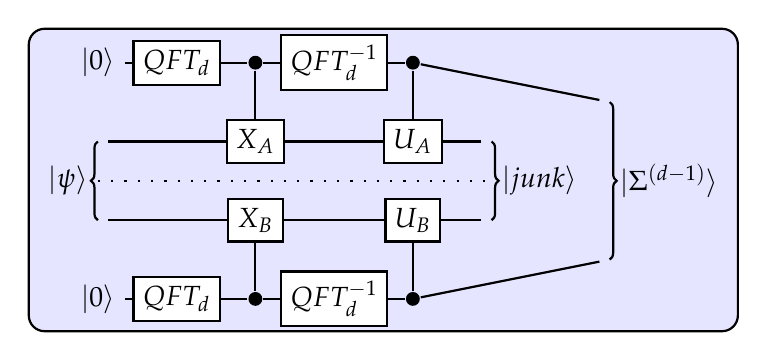
\begin{tikzpicture}[thick]
        %
        % `operator' will only be used by Hadamard (H) gates here.
        % `phase' is used for controlled phase gates (dots).
        % `surround' is used for the background box.
        \tikzstyle{operator} = [draw,fill=white,minimum size=1.5em] 
        \tikzstyle{phase} = [fill,shape=circle,minimum size=5pt,inner sep=0pt]
        \tikzstyle{surround} = [fill=blue!10,thick,draw=black,rounded corners=2mm]
        %
        % Bracket
        \draw[decorate,decoration={brace,mirror},thick] (0,-1) to
    	node[midway,left] (bracket1) {$\ket{\psi}$}
    	(0,-2);
        % Qubits
        \node at (0,0) (q1) {$\ket{0}$};
        \node at (0,-1) (q2) {};
        \node at (0,-2) (q3) {};
        \node at (0,-3) (q4) {$\ket{0}$};
        %
        % Column 1
        \node[operator] (op11) at (1,0) {$QFT_d$} edge [-] (q1);
        \node[operator] (op14) at (1,-3) {$QFT_d$} edge [-] (q4);
        %
        % Column 3
        \node[phase] (phase11) at (2,0) {} edge [-] (op11);
	\node[operator] (op22) at (2,-1) {$X_A$} edge [-] (q2);
	\node[operator] (op23) at (2, -2) {$X_B$} edge[-] (q3);
        \node[phase] (phase14) at (2,-3) {} edge [-] (op14);
        \draw[-] (phase11) -- (op22);
        \draw[-] (phase14) -- (op23);
        %
        % Column 4
        \node[operator] (op31) at (3,0) {$QFT_d^{-1}$} edge [-] (phase11);
        \node[operator] (op34) at (3,-3) {$QFT_d^{-1}$} edge [-] (phase14);
        %
        % Column 5
        \node[phase] (phase21) at (4,0) {} edge [-] (op31);
	\node[operator] (op42) at (4,-1) {$U_A$} edge [-] (op22);
	\node[operator] (op43) at (4, -2) {$U_B$} edge[-] (op23);
        \node[phase] (phase24) at (4,-3) {} edge [-] (op34);
        \draw[-] (phase21) -- (op42);
        \draw[-] (phase24) -- (op43);
        %
        % Column 6
        \node (end2) at (5,-1) {} edge [-] (op42);
        \node (end3) at (5,-2) {} edge [-] (op43);
        %
        % Bracket
        \draw[decorate,decoration={brace},thick] (5,-1) to
    	node[midway,right] (bracket) {$\ket{junk}$}
    	(5,-2);
        %
        % Column 7
        \node (end1) at (6.5,-0.5) {} edge [-] (phase21);
        \node (end4) at (6.5,-2.5) {} edge [-] (phase24);
        % Dashed line
        \draw[loosely dotted] (0,-1.5) -- (5,-1.5);
        % Bracket
        \draw[decorate,decoration={brace},thick,] (6.5,-0.5) to
    	node[midway,right] (bracket2) {$\ket{\EPR{d-1}}$}
    	(6.5,-2.5);
        %
        % Background Box
        \begin{pgfonlayer}{background} 
        \node[surround] (background) [fit = (q1) (op14) (bracket1)(bracket2)] {};
        \end{pgfonlayer}
        %
        \end{tikzpicture}
	\caption{The isometries $\Phi_A$ and $\Phi_B$.}
\end{figure}
The isometry maps the state $\ket{\psi}$ in the following steps:
\begin{enumerate}
	\item Append $\ket{0}_A$ on Alice's side and $\ket{0}_B$ on Bob's side as control registers, and
	the state becomes $\ket{\psi} \ket{0}_A \ket{0}_B$;
	\item Apply $QFT_d$ to the control registers, and the state becomes
	\begin{align}
		\frac{1}{d} \sum_{k_1,k_2 =0}^{d-1} \ket{\psi} \ket{k_1}_A \ket{k_2}_B;
	\end{align}
	\item Apply $X_A^{k_1}$ to Alice's share of $\ket{\psi}$ and $X_B^{k_2}$ to Bob's share controlled
	by the control registers, and the state becomes
	\begin{align}
		&\frac{1}{d} \sum_{k_1,k_2 =0}^{d-1}X_A^{k_1} X_B^{k_2}\ket{\psi} \ket{k_1}_A \ket{k_2}_B\\
		=&\frac{1}{d} \sum_{k_1,k_2 =0}^{d-1} \sum_{i=1}^{d-1}\sum_{j=1}^m c_j X_A^{k_1}\ket{x_{i,j}}_A X_B^{k_2}\ket{x_{i,j}}_B
		\ket{k_1}_A \ket{k_2}_B\\
		=&\frac{1}{d} \sum_{k_1,k_2 =0}^{d-1} \sum_{i=1}^{d-1}\sum_{j=1}^m c_j \omega_d^{k_1i+k_2i} \ket{x_{i,j}}_A\ket{x_{i,j}}_B
		\ket{k_1}_A \ket{k_2}_B;
	\end{align}
	\item Apply $QFT_d^{-1}$ to the control registers, and the state becomes
	\begin{align}
		&\frac{1}{d^2} \sum_{l_1,l_2 =0}^{d-1}\sum_{i=1}^{d-1}\sum_{j=1}^m c_j \omega_d^{k_1(i-l_1)+k_2(i-l_2)} \ket{x_{i,j}}_A\ket{x_{i,j}}_B
		\ket{l_1}_A \ket{l_2}_B\\
		=& \sum_{i=1}^{d-1}\sum_{j=1}^m c_j \ket{x_{i,j}}_A\ket{x_{i,j}}_B \ket{i}_A \ket{i}_B;
	\end{align}
	\item Let $n_i$ satisfy the condition $r^{n_i} \equiv i \pmod{d}$, apply $U_A^{(i)} = U_A^{n_i}$ to Alice's share of $\ket{\psi}$ and $U_B^{(i)} = U_B^{n_i}$ to Bob's share controlled
	by the control registers, and the state becomes
	\begin{align}
		&\sum_{i=1}^{d-1}\sum_{j=1}^m c_j U_A^{(i)}\ket{x_{i,j}}_A U_B^{(i)}\ket{x_{i,j}}_B \ket{i}_A\ket{i}_B \\
		=&\sum_{i=1}^{d-1} \sum_{j=1}^m c_j \ket{x_{i r^{-n_i} ,j}}_A \ket{x_{i r^{-n_i},j}}_B \ket{i}_A\ket{i}_B\\
		=& \sum_{i=1}^{d-1} \sum_{j=1}^m c_j \ket{x_{i i^{-1},j}}_A \ket{x_{i i^{-1},j}}_B \ket{i}_A\ket{i}_B\\
		= &\left(\sum_{j=1}^m c_j \ket{x_{1,j}}_A \ket{x_{1,j}}_B\right) \x \sum_{i=1}^{d-1} \ket{i}_A\ket{i}_B\\
		=&\sqrt{d-1} \left(\sum_{j=1}^m c_j \ket{x_{1,j}}_A \ket{x_{1,j}}_B\right) \x 
		\frac{1}{\sqrt{d-1}}\sum_{i=1}^{d-1}\ket{i}_A\ket{i}_B\\
		=&\sqrt{d-1} \left(\sum_{j=1}^m c_j \ket{x_{1,j}}_A \ket{x_{1,j}}_B\right) \x \ket{\EPR{d-1}},
	\end{align}
	where in the last line we used the fact that $\norm{\sum_{j=1}^m c_j \ket{x_{1,j}}_A \ket{x_{1,j}}_B} = 1/\sqrt{d-1}$.
\end{enumerate}

If the initial state is $X_A\ket{\psi}$, the isometry maps the state as following
\begin{align}
	X_A\ket{\psi} \to &X_A\ket{\psi}\ket{0}_A\ket{0}_B\\
	\to &\frac{1}{d} \sum_{k_1,k_2 =0}^{d-1} X_A\ket{\psi} \ket{k_1}_A \ket{k_2}_B \\
	\to &\frac{1}{d} \sum_{k_1,k_2 =0}^{d-1} X_A^{k_1+1} X_B^{k_2}\ket{\psi} \ket{k_1}_A \ket{k_2}_B \\
	=&\frac{1}{d} \sum_{k_1,k_2 =0}^{d-1} \sum_{i=1}^{d-1}\sum_{j=1}^m c_j \omega_d^i\omega_d^{(k_1+k_2)i} \ket{x_{i,j}}_A\ket{x_{i,j}}_B
		\ket{k_1}_A \ket{k_2}_B\\
	\to &\frac{1}{d^2}\sum_{k_1,k_2 =0}^{d-1} \sum_{i=1}^{d-1}\sum_{j=1}^m c_j \omega_d^i\omega_d^{(k_1-l_1)i+(k_2-l_2)i} \ket{x_{i,j}}_A\ket{x_{i,j}}_B
		\ket{l_1}_A \ket{l_2}_B\\
	=&\sum_{i=1}^{d-1}\sum_{j=1}^m c_j \omega_d^i \ket{x_{i,j}}_A\ket{x_{i,j}}_B \ket{i}_A \ket{i}_B\\
	\to& \sum_{i=1}^{d-1}\sum_{j=1}^m c_j \omega_d^i U_A^{(i)}\ket{x_{i,j}}_A U_B^{(i)}\ket{x_{i,j}}_B \ket{i}_A\ket{i}_B\\
	=&\sum_{i=1}^{d-1}\sum_{j=1}^m c_j \omega_d^i \ket{x_{1,j}}_A \ket{x_{1,j}}_B \ket{i}_A\ket{i}_B\\
	=&\sqrt{d-1} \left(\sum_{j=1}^m c_j \ket{x_{1,j}}_A \ket{x_{1,j}}_B\right) \x 
		\frac{1}{\sqrt{d-1}} \sum_{i=1}^{d-1}\omega_d^i \ket{i}_A\ket{i}_B\\
	=& \sqrt{d-1} \left(\sum_{j=1}^m c_j \ket{x_{1,j}}_A \ket{x_{1,j}}_B\right) \x \tX_A \ket{\EPR{d-1}},
\end{align}
where $\tX_A$ is the ideal $X$ operator.
The case of $X_B\ket{\psi}$ is similar, so we omit it here. 

If the initial state is $U_A\ket{\psi}$, the isometry maps the state as following
\begin{align}
	U_A\ket{\psi} \to &U_A\ket{\psi}\ket{0}_A\ket{0}_B\\
	\to &\frac{1}{d} \sum_{k_1,k_2 =0}^{d-1} U_A\ket{\psi} \ket{k_1}_A \ket{k_2}_B \\
	= &\frac{1}{d} \sum_{k_1,k_2=0}^{d-1} \sum_{i=1}^{d-1}\sum_{j=1}^m c_j U_A\ket{x_{i,j}}_A\ket{x_{i,j}}_B
		\ket{k_1}_A \ket{k_2}_B\\
	= & \frac{1}{d} \sum_{k_1,k_2=0}^{d-1} \sum_{i=1}^{d-1}\sum_{j=1}^m c_j \ket{x_{i r^{-1} ,j}}_A\ket{x_{i,j}}_B
		\ket{k_1}_A \ket{k_2}_B\\
	\to &\frac{1}{d} \sum_{k_1,k_2 =0}^{d-1} \sum_{i=1}^{d-1}\sum_{j=1}^m c_j X_A^{k_1} \ket{x_{i r^{-1} ,j}}_A
	X_B^{k_2}\ket{x_{i,j}}_B  \ket{k_1}_A \ket{k_2}_B \\
	=&\frac{1}{d} \sum_{k_1,k_2 =0}^{d-1} \sum_{i=1}^{d-1}\sum_{j=1}^m c_j \omega_d^{k_1 i/r}\omega_d^{k_2i} \ket{x_{ir^{-1},j}}_A\ket{x_{i,j}}_B
		\ket{k_1}_A \ket{k_2}_B\\
	\to &\frac{1}{d^2}\sum_{k_1,k_2 =0}^{d-1} \sum_{i=1}^{d-1}\sum_{j=1}^m c_j \omega_d^{k_1(i/r-l_1)}\omega_d^{(k_2(i-l_2)} \ket{x_{ir^{-1},j}}_A\ket{x_{i,j}}_B
		\ket{l_1}_A \ket{l_2}_B\\
	=&\sum_{i=1}^{d-1}\sum_{j=1}^m c_j  \ket{x_{ir^{-1},j}}_A\ket{x_{i,j}}_B \ket{ir^{-1}}_A \ket{i}_B\\
	\to& \sum_{i=1}^{d-1}\sum_{j=1}^m c_j U_A^{(ir^{-1})}\ket{x_{ir^{-1},j}}_A U_B^{(i)}\ket{x_{i,j}}_B \ket{i}_A\ket{i}_B\\
	=&\sum_{i=1}^{d-1}\sum_{j=1}^m c_j \ket{x_{1,j}}_A \ket{x_{1,j}}_B \ket{ir^{-1}}_A\ket{i}_B\\
	=&\sqrt{d-1} \left(\sum_{j=1}^m c_j \ket{x_{1,j}}_A \ket{x_{1,j}}_B\right) \x 
		\frac{1}{\sqrt{d-1}} \sum_{i=1}^{d-1}\ket{ir^{-1}}_A\ket{i}_B\\
	=& \sqrt{d-1} \left(\sum_{j=1}^m c_j \ket{x_{1,j}}_A \ket{x_{1,j}}_B\right) \x \tU_A \ket{\EPR{d-1}},
\end{align}
where $\tU_A$ is the ideal $U$ operator on Alice's side.
The derivation is similar when $U_B$ is applied, so we omit it here.
\end{proof}
%The effect of $\CHSH_X$ and $\SVT_X$ is that we have a set $\{ \ket{x_i} \}_{i \in [d]} \in \supp(\rho_A)$ such that
%\begin{align}
%	X \ket{x_i} = \omega_d^i \ket{x_i}.
%\end{align}
%The other effect of $\SVT_X$ is that we know 
%\begin{align}
%	\tA_\triangle^\diamond \rho_A \tA_\triangle^\diamond = \frac{1}{d} \ketbra{x_0}{x_0} = \frac{1}{d} \tA_\triangle^\diamond.
%\end{align}
%\hl{\textbf{Question}: Can we show $\Tr(\ketbra{x_2}{x_2} \rho_A) = 1/d$?}
In summary, for any odd prime number $d$ whose primitive root is $2$,$3$ or $5$, 
\cref{prop:realize} tells us that the correlation $C(d)$ is achievable by a quantum strategy 
and \cref{thm:selftest} tells us that the correlation $C(d)$ can self-test the EPR pair of
local dimension $d-1$. Moreover, there are infinitely many prime numbers
whose primitive root is in the set $\{2,3,5\}$ \cite{murty1988},
Hence, our main result is the following theorem.
\begin{theorem}
	There exists an infinity-sized set $D$ of prime numbers such that 
	each $d \in D$ has primitive root $2$, $3$ or $5$ and there exists
	a constant-sized correlation $C(d)$ that can self-test the EPR pair of 
	local dimension $d-1$.
\end{theorem}
We remark that our proof works for any odd prime number with primitive root $r$.
However, since there is no upper-bound of $r$ for a general prime number $d$, we 
cannot claim the corresponding correlation $C(d)$ is constant-sized. On the other
hand, since $r$ is usually much smaller than $d$, our result implies a more efficient
way to test EPR pairs of prime local dimension than the one proposed in Ref.~\cite{cgs2017}.
The size of our correlation grows linearly in $r$ whereas the Coladangelo \textit{et. al.}'s
method uses correlation grows linearly in $d$.

\bibliographystyle{alphaurl}
\bibliography{quantum_correlation}
\appendix
%========================================
\section{The proof of \cref{thm:selftest} }
\label{sec:selftest}
%========================================
This proof follows the same line of argument in Appendix A of Ref.~\cite{bamps2015}.
We first find two sum-of-square decompositions of $2\sqrt{\alpha^2+1} \1 - \I_\alpha$,
where $\I_\alpha$ is expressed in terms of $\{M_x\}$ and $\{N_y\}$.
The decompositions allow us to determine some key relations between Alice and Bob's observables
and their shared state, which will be used to draw the conclusion.

\begin{proof}
The first step is to find a sum-of-square decomposition of 
the following Bell expression
\begin{align}
	\bar{\I}_\alpha = 2\sqrt{\alpha^2+1} \1 - \I_\alpha
	= \frac{2}{\sin(\mu)} \1 - \frac{\cos(\mu)}{\sin(\mu)}(M_1N_1+M_1N_2) -  M_2N_1 + M_2N_2.
\end{align} 
With the notation $c:= \cos(\mu)$, $s := \sin(\mu)$ and 
\begin{align*}
	&Z_A = M_1 && X_A = M_2\\
	&Z_B = \frac{N_1+N_2}{2c} && X_B = \frac{N_1-N_2}{2s},
\end{align*}
the two SOS decompositions that we use are
\begin{align}
	\label{eq:sos1}&\bar{\I}_\alpha = \frac{s \bar{\I}_\alpha^2 + 4sc^2(Z_AX_B+X_AZ_B)^2}{4},\\
	\label{eq:sos2}&\bar{\I}_\alpha = \frac{c^2}{s}(Z_A-Z_B)^2 + s(X_A-X_B)^2.
\end{align}
The verification is omitted here. From the SOS decomposition, we establish \cref{eq:za-zb,eq:xa-xb,eq:xazb,eq:zaxb,eq:zaxa,eq:zaxaxbzb}.
We define
\begin{align*}
	&S_1 = \frac{\sqrt{s}}{2} \bar{\I}_\alpha, &&
	S_2 = \sqrt{s}c(Z_AX_B+ X_AZ_B),\\
	&S_3 = \frac{c}{\sqrt{s}}(Z_A-Z_B), &&
	S_4 = \sqrt{s}(X_A-X_B)
\end{align*}
then 
\begin{align}
\bar{\I}_\alpha = S_1^2 + S_2^2 = S_3^2 + S_4^2
\end{align}
The fact that the quantum strategy $(\ket{\psi}, \{M_x\}_{x=1,2}, \{N_{y }\}_{y=1,2}$ achieves that 
$\ip{\bar{\I}_\alpha} \leq \epsilon$ implies that
$\bra{\psi} S_i^2 \ket{\psi} \leq \ep$, and equivalently, $\norm{S_i \ket{\psi}} \leq \se$ for $i = 1,2,3,4$.
From the definitions of $S_i$'s, we can get that 
\begin{align}
	&\norm{(X_AZ_B+X_BZ_A)\ket{\psi}} \leq \frac{1}{c\sqrt{s}} \se\\
	&\norm{(Z_A-Z_B)\ket{\psi}} \leq \frac{\sqrt{s}}{c} \se\\
	&\norm{(X_A-X_B)\ket{\psi}} \leq \frac{1}{\sqrt{s}} \se.
\end{align}
The first and the second inequality give us that 
\begin{align}
	\norm{ [Z_A(\1+X_B) - (\1-X_A)Z_B] \ket{\psi} } 
	\leq \norm{(X_AZ_B+X_BZ_A)\ket{\psi}} + \norm{(Z_A-Z_B)\ket{\psi}}
	\leq \frac{s+1}{c\sqrt{s}} \se.
\end{align}
Similarly, the first and the third inequality give us that 
\begin{align}
	\norm{[X_A(\1+Z_B) - X_B(\1-Z_A)] \ket{\psi}} \leq \frac{c+1}{c\sqrt{s}} \se.
\end{align}
Since $Z_AX_A +X_A Z_A = \frac{S_2}{c\sqrt{s}} + \frac{\sqrt{s}\tilde{X}_AS_3}{c} + \frac{\tilde{Z}_AS_4}{\sqrt{s}}$, we can deduce that
\begin{align}
	\norm{ (Z_A X_A+X_AZ_A)\ket{\psi}} \leq \frac{1+c+s}{c\sqrt{s}} \se.
\end{align}
To prove \cref{eq:zaxaxbzb}, we switch to the approximate relation form and derive that 
\begin{align}
	X_AZ_A \ket{\psi} &\appd{\frac{1+c+s}{c\sqrt{s}} \se}  -Z_AX_A \ket{\psi} \\
	&\appd{\frac{\sqrt{s}}{c} \se} -Z_AX_B \ket{\psi} \\
	&\appd{\frac{1}{s^{3/2} }\se} -X_BZ_B\ket{\psi},
\end{align}
where in the last line we use the fact $\norm{X_B} \leq 1/s$.

Now we introduce the isometries $\Phi_A$ and $\Phi_B$ mentioned in the statement of the theorem.
They are the same as the ones used in Ref.~\cite{bamps2015}.
To construct $\Phi_A$ and $\Phi_B$ we need to regularize $Z_B$ and $X_B$ to make sure the corresponding operations 
are unitary in the isometries. We define $Z_B^\ast$ to be the operator obtained from $Z_B$ by changing all the $0$-eigenvalues
to $1$ and 
\begin{align*}
Z_B' := Z_B^\ast |Z_B^\ast|^{-1},
\end{align*}
where $|Z_B^\ast|$ is obtained from $Z_B^\ast$ by replacing all negative eigenvalues by its absolute value.
In a similar way, we define $X_B^\ast$ and $X_B'$.
On Alice's side, since $Z_A$ and $X_A$ are unitaries already,
we define
$Z_A' := Z_A$ and $X_A' = X_A$.
The isometries are illustrated in the figure below.
\begin{figure}[H]
\center
        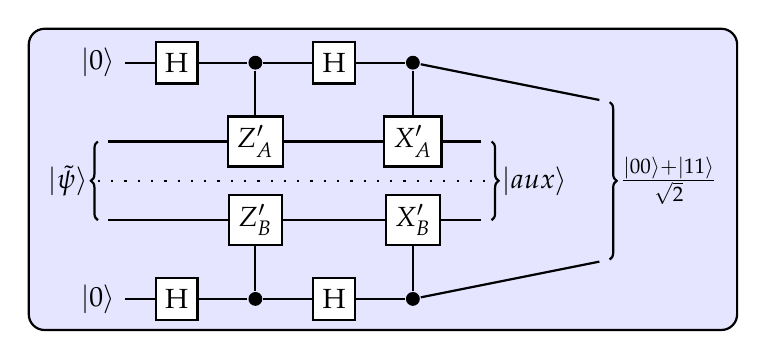
\begin{tikzpicture}[thick]
        %
        % `operator' will only be used by Hadamard (H) gates here.
        % `phase' is used for controlled phase gates (dots).
        % `surround' is used for the background box.
        \tikzstyle{operator} = [draw,fill=white,minimum size=1.5em] 
        \tikzstyle{phase} = [fill,shape=circle,minimum size=5pt,inner sep=0pt]
        \tikzstyle{surround} = [fill=blue!10,thick,draw=black,rounded corners=2mm]
        %
        % Bracket
        \draw[decorate,decoration={brace,mirror},thick] (0,-1) to
    	node[midway,left] (bracket1) {$\ket{\tpsi}$}
    	(0,-2);
        % Qubits
        \node at (0,0) (q1) {$\ket{0}$};
        \node at (0,-1) (q2) {};
        \node at (0,-2) (q3) {};
        \node at (0,-3) (q4) {$\ket{0}$};
        %
        % Column 1
        \node[operator] (op11) at (1,0) {H} edge [-] (q1);
        \node[operator] (op14) at (1,-3) {H} edge [-] (q4);
        %
        % Column 3
        \node[phase] (phase11) at (2,0) {} edge [-] (op11);
	\node[operator] (op22) at (2,-1) {$Z_A'$} edge [-] (q2);
	\node[operator] (op23) at (2, -2) {$Z_B'$} edge[-] (q3);
        \node[phase] (phase14) at (2,-3) {} edge [-] (op14);
        \draw[-] (phase11) -- (op22);
        \draw[-] (phase14) -- (op23);
        %
        % Column 4
        \node[operator] (op31) at (3,0) {H} edge [-] (phase11);
        \node[operator] (op34) at (3,-3) {H} edge [-] (phase14);
        %
        % Column 5
        \node[phase] (phase21) at (4,0) {} edge [-] (op31);
	\node[operator] (op42) at (4,-1) {$X_A'$} edge [-] (op22);
	\node[operator] (op43) at (4, -2) {$X_B'$} edge[-] (op23);
        \node[phase] (phase24) at (4,-3) {} edge [-] (op34);
        \draw[-] (phase21) -- (op42);
        \draw[-] (phase24) -- (op43);
        %
        % Column 6
        \node (end2) at (5,-1) {} edge [-] (op42);
        \node (end3) at (5,-2) {} edge [-] (op43);
        %
        % Bracket
        \draw[decorate,decoration={brace},thick] (5,-1) to
    	node[midway,right] (bracket) {$\ket{aux}$}
    	(5,-2);
        %
        % Column 7
        \node (end1) at (6.5,-0.5) {} edge [-] (phase21);
        \node (end4) at (6.5,-2.5) {} edge [-] (phase24);
        % Dashed line
        \draw[loosely dotted] (0,-1.5) -- (5,-1.5);
        % Bracket
        \draw[decorate,decoration={brace},thick,] (6.5,-0.5) to
    	node[midway,right] (bracket2) {$\frac{\ket{00}+\ket{11}}{\sqrt{2}}$}
    	(6.5,-2.5);
        %
        % Background Box
        \begin{pgfonlayer}{background} 
        \node[surround] (background) [fit = (q1) (op14) (bracket1)(bracket2)] {};
        \end{pgfonlayer}
        %
        \end{tikzpicture}
	\caption{The isometries $\Phi_A$ and $\Phi_B$.}
\end{figure}
To bound $e_{xy} := \norm{ (\Phi_A\x\Phi_B) (\tA_x \x \tB_y) \ket{\tpsi} - \ket{junk} \x (A_x\x B_y) \ket{\EPR{2}}}$,
there are some intermediate steps. Since the derivations are the same as in Ref.~\cite{bamps2015}, 
we only record the key relations here.
\begin{align*}
	&\norm{(Z_B' - Z_B) \ket{\tpsi}} \leq \frac{\sqrt{s}}{c} \sqrt{\epsilon},\\
	&\norm{(Z_B' - Z_A') \ket{\tpsi}} \leq 2 \frac{\sqrt{s}}{c}\sqrt{\epsilon}, \\
	&\norm{(X_B' - X_B) \ket{\tpsi}} \leq \frac{c+1}{s^{3/2}} \sqrt{\epsilon} := \delta_1 \sqrt{\epsilon},\\
	&\norm{(X_B'Z_B'+ Z_B'X_B')\ket{\tpsi}} \leq [\frac{2\sqrt{s}}{c} + \frac{2}{\sqrt{s}} + 2\delta_1 + 
	(\sqrt{2}+\frac{1}{c})(2\frac{\sqrt{s}}{c}+\frac{1+c+s}{c\sqrt{s}})]\sqrt{\epsilon}
	:= \delta_2 \sqrt{\epsilon}.
\end{align*}
Then we can calculate that 
\begin{align*}
	&e_{00} = e_{10} = 2\delta_2 \sqrt{\epsilon}\\
	&e_{20} = 2(\frac{1+c+s}{c\sqrt{s}} + \delta_2) \sqrt{\epsilon}\\
	&e_{01} = e_{02} = e_{11} = e_{12} = [\sqrt{s}+s(2\frac{1+c+s}{c\sqrt{s}} + \delta_1) + 2\delta_2]\sqrt{\epsilon}\\
	&e_{21} = e_{22} = [2\frac{1+c+s}{c\sqrt{s}} + \sqrt{s}+s(2\frac{1+c+s}{c\sqrt{s}} + \delta_1) + 2\delta_2]\sqrt{\epsilon},
\end{align*}
so an upper bound of the error is that
\begin{align}
	\forall x,y \in \{0,1,2\}, e_{xy} \in O((\frac{1}{c^2s^{1/2}} + \frac{1}{s^{3/2}})\sqrt{\epsilon}).
\end{align}
\end{proof}
%%=====================================
\section{The proof of \cref{lm:uo_independ}}
\label{sec:u_and_o}
%%=====================================

We are going to prove 
the set $\{U^k O^l\}$ for $k=0,1\dots d-2$ and $l = 1,2\dots d-1$ forms a basis of the ring of $(d-1)\times (d-1)$ matrices over $\C$
Note that the unitaries $U$ and $O$ defined in the lemma above satisfy the condition $UOU^\dagger = O^r$.
In this proof, we denote the set $\{0,1,2\dots d-2\}$ by $[d-1]$ and the set $\{1,2 \dots d-1\}$ by $[d-1]+1$.
\begin{proof}
We are going to show the $(d-1)^2$ matrices from the set $\{U^k O^l\}_{k \in[d-1], l \in [d-1]+1}$ are linearly independent.
Suppose there exists a set of complex numbers $\{ x_{k,l} \}_{k \in[d-1], l \in [d-1]+1}$
such that 
\begin{align}
	M = \sum_{k=0}^{d-2} \sum_{l=1}^{d-1} x_{k,l} U^k O^l = 0. 
\end{align}
We \hf{define} a set of integers $\{ k_i \}_{i=1}^{d-1}$ such that $r^{k_i} \equiv i \pmod{d}$.
\carl{We shouldn't be making extra assumptions that are not stated in the lemma.  This looks to me more like
a definition of the variables $\{ k_i \}$, rather than an assumption.}
The fact that $r$ is a primitive root of $d$ guarantees that $k_i$'s are distinct.
Then we can group $\{x_{k,l}\}$ into vectors: $\ket{x_{k_1}}, \ket{x_{k_2}} \dots \ket{x_{k_{d-1}}}$,
where $\ket{x_{k_i}}= (x_{k_i, 1}, x_{k_i, 2} \dots x_{k_i, d-1})^\intercal$.
Our goal is equivalent to proving that $\ket{x_{k_i}} = 0$ for all $i$.

We start with proving that $\ket{x_{k_1}} = 0$.
Proving $\ket{x_{k_i}} = 0$ for other $i$ follows a similar argument, so we briefly
discuss about it in the end.
The entry $\bra{1}M\ket{1}$ can be expressed as  
\begin{align}
	\bra{1}M\ket{1} = \sum_{k=0}^{d-2}\sum_{l = 1}^{d-1}\sum_{i=1}^{d-1} x_{k, l}\omega_d^{il}\braket{1}{i (r^{-1})^k}\braket{i}{1}.
\end{align}
For the term $\braket{1}{i (r^{-1})^k}\braket{i}{1} \neq 0$ we must have $i = 1$ and $r^k \equiv 1 \pmod{d}$, or equivalently,
$k = k_1$. We can conclude that 
\begin{align}
	\bra{1}M\ket{1} = \sum_{l = 1}^{d-1} x_{k_1,l}\omega_d^l = 0. 
\end{align}
Similarly we can determine that for all $j = 1,2\dots d-1$,
\begin{align}
	\bra{j}M\ket{j} 
	=  \sum_{k=0}^{d-2}\sum_{l = 1}^{d-1}\sum_{i=1}^{d-1} x_{k, l}\omega_d^{il}\braket{j}{i (r^{-1})^k}\braket{i}{j} 
	= \sum_{l = 1}^{d-1}x_{k_1,l}\omega_d^{jl} = 0.
\end{align}
Hence we get $d-1$ equations with $d-1$ variables, and the linear system is
\begin{align}
	W \ket{x_{k_1}} = 0,
\end{align}
where $W(m,n) = \omega_d^{mn}$. Then we define
\begin{align}
	\tW = 
	\begin{pmatrix}
	1 & 1 \\
	1 & W
	\end{pmatrix}.
\end{align}
First observe that $\tW$ is a Vandermonde matrix, hence it is non-singular.
Next, we define $\ket{\tx_{k_1}} = (0, x_{k_1,1}, \dots x_{k_1,d-1})^\intercal$ 
and prove that it satisfies the condition
that 
\begin{align}
	\tW \ket{\tx_{k_1}} = 0,
\end{align}
which involves $d$ equations. The last $d-1$ equations are given by the assumption and $M$.
We only need to prove that $\sum_{l=1}^d x_{k_1, l} = 0$, which is required by the first row of $\tW$.
It can be proved by summing the known $d-1$ equations as follows
\begin{align}
	0=\sum_{j = 1}^{d-1} \bra{j}M\ket{j}  
	=  \sum_{j=1}^{d-1}\sum_{l = 1}^{d-1}x_{k_1,l}\omega_d^{jl}
	=\sum_{l = 1}^{d-1}x_{k_1,l} (\sum_{j=1}^{d-1} \omega_d^{jl})
	= \sum_{l = 1}^{d-1}- x_{k_1,l}
\end{align}
where we have used the fact that $\sum_{j=1}^{d-1} \omega_d^{jl} =-1$ for all $l = 1,2\dots d-1$.
Since $\tW$ is non-singluar, we know $\ket{\tx_{k_1}} = 0$ which implies that $\ket{x_{k_1}} = 0$.

For $\ket{x_{k_a}}$, we look at entries $\{\bra{j}M\ket{aj}\}_{j=1}^{d-1}$ for $a = 2 \dots d-1$ and get equations
of the form
\begin{align}
	0 = \bra{j}M\ket{aj} = \sum_{l=1}^{d-1} x_{k_a, l} \omega_d^{ajl} 
\end{align}
The corresponding coefficient matrix has value $\omega_d^{amn}$ at coordinate $(m,n)$,
so it is also a submatrix of a Vandermonde matrix. Similar argument gives us that $\ket{x_{k_a}} = 0$.

To summarize, we have proven that $x_{k,l} = 0$ for all $k$ and $l$, which implies that the elements of the set
$\{ U^k X^l \}$ are linearly independent and forms a basis for the ring of all the $(d-1)\times(d-1)$ matrices over $\C$.
\carl{Nice proof.  I like the use of the Vandermonde matrix.  We can think a little about possible simplifications.}
\end{proof}


\end{document}
